%%
%% Arquivo principal para:
%% - teses de doutorado
%% - dissertaes de mestrado
%% - exames de qualificao de mestrado e doutorado
%%
%% NOTA: A PUBLICAO DESTE MODELO VISA APENAS ORIENTAR OS PS-GRADUANDOS
%% NA PREPARAO DE SEUS TEXTOS. O PPgEE DA UFRN NO PROV ASSISTNCIA NO
%% USO DAS FERRAMENTAS NECESSRIAS AO USO DESTE MODELO (LATEX, XFIG, ETC.)
%% 1
%% Adelardo Medeiros, dezembro de 2005.

% DEFINIES GLOBAIS
% Esta primeira linha d informaes gerais sobre o documento.
% PARA A VERSO FINAL:
% papel A4, letra grande (12pt), openr	sight (captulos s iniciam em
% pgina direita, se necessrio incluindo uma pgina em branco),
% twoside (o documento vai ser impresso em frente e costa)
%\documentclass[a4paper,12pt,openright,twoside]{book}
% PARA A QUALIFICAO E PARA A VERSO INICIAL:
% papel A4, letra grande (12pt), openany (captulos iniciam em
% qualquer pgina), oneside (o documento vai ser impresso s na frente)
\documentclass[a4paper,12pt,openany,oneside]{book}

% PACOTES OBRIGATRIOS
\usepackage{epigraph}
\usepackage{setspace}

%\usepackage{lipsum}
% Use estes pacotes para poder digitar diretamente as letras com acento
% e para que a hifenizao funcione corretamente
%\usepackage[latin1]{inputenc}
\usepackage[utf8]{inputenc}
\usepackage{ae}
% Para usar fontes standard ao invs das do LaTeX (gera melhores PDFs)
\usepackage{pslatex}
% Para a hifenizao em portugus
\usepackage[portuges, brazil]{babel}


% Para que os primeiros pargrafos das sees tambm sejam indentados
\usepackage{indentfirst}
% Para poder incluir grficos (figuras)
\usepackage{graphicx}
% Para poder fazer glossrio ou lista de smbolos
% Use a segunda opo se quiser incluir na definio do smbolo a
% pgina e/ou a equao onde ela foi definida
\usepackage[portuguese,noprefix]{nomencl}
%\usepackage[portuguese,noprefix,refeq,refpage]{nomencl}
% Para permitir espaamento simples, 1 1/2 e duplo
\usepackage{setspace}
% Para usar alguns comandos matemticos avanados muito teis
\usepackage{amsmath}
% Para poder usar o ambiente "comment"
\usepackage{verbatim}
% Para poder ter tabelas com colunas de largura auto-ajustvel
\usepackage{tabularx}
% Para executar um comando depois do fim da pgina corrente
\usepackage{afterpage}
% Para formatar URLs (endereos da Web)
\usepackage{url}
% Para reduzir os espaos entre os tens (itemize, enumerate, etc.)
% Este pacote no faz parte da distribuio padro do LaTeX.
\usepackage{noitemsep}
% Para as citaes bibliogrficas
\usepackage[abbr]{harvard}	% As chamadas so sempre abreviadas
\harvardparenthesis{square}	% Colchetes nas chamadas
%\harvardyearparenthesis{round}	% Parntesis nos anos das referncias
\renewcommand{\harvardand}{e}	% Substituir "&" por "e" nas referncias

% PACOTES OPCIONAIS

% Para poder incluir arquivos Postscript com cores (do Xfig, por exemplo)
\usepackage{color}
% Para ter clulas em tabelas que ocupam mais de uma linha
\usepackage{multirow}
\usepackage[table,xcdraw]{xcolor}
% Para poder ter tabelas longas em mais de uma pgina
%\usepackage{longtable}
% Para poder escrever partes do texto em "n" colunas
%\usepackage{multicol}
% Se voc quiser personalizar os cabealhos das pginas
%\usepackage{fancyheadings}
% Para incluir algoritmos e listagens de cdigos
\usepackage{listings}
% Captulos com ttulos em um formato "decorado"
\usepackage{capitulos}

\hyphenation{skinRGBDetect}

%FIGURAS LADO A LADO
\usepackage{subfigure}

% NOVOS COMANDOS

% As definies dos novos comandos esto agrupadas no arquivo "comandos.tex"
% Esta separao  opcional: se voc preferir, pode por as definies
% diretamente neste arquivo
% newcommand define novos comandos, que podem passar a ser usados da
% mesma forma que os comandos LaTeX de base.

% Implica��o em f�rmulas
\newcommand{\implica}{\quad\Rightarrow\quad} %Meio de linha
\newcommand{\implicafim}{\quad\Rightarrow}   %Fim de linha
\newcommand{\tende}{\rightarrow}
\newcommand{\BibTeX}{\textsc{B\hspace{-0.1em}i\hspace{-0.1em}b\hspace{-0.3em}}\TeX}

% Fra��o com parentesis
\newcommand{\pfrac}[2]{\left(\frac{#1}{#2}\right)}

% Transformada de Laplace e transformada Z
%\newcommand{\lapl}{\makebox[0cm][l]{\hspace{0.1em}\raisebox{0.25ex}{-}}\mathcal{L}}
\newcommand{\lapl}{\pounds}
\newcommand{\transfz}{\mathcal{Z}}

% N�o aparecer o n�mero na primeira p�gina dos cap�tulos
\newcommand{\mychapter}[1]{\chapter{#1}\thispagestyle{empty}}

% Os cap�tulos sem n�mero
\newcommand{\mychapterast}[1]{\chapter*{#1}\thispagestyle{empty}
\chaptermark{#1}
\afterpage{\markboth{\uppercase{#1}}{\rightmark}}
\markboth{\uppercase{#1}}{}
}

% Se��es sem n�mero
\newcommand{\mysectionast}[1]{\section*{#1}
\addcontentsline{toc}{section}{#1}
\markright{\uppercase{#1}}
}

% No tabularx, as celulas devem ser centradas verticalmente
\renewcommand{\tabularxcolumn}[1]{m{#1}}

% C�lulas centralizadas horizontalmente no tabularx
\newcolumntype{C}{>{\centering\arraybackslash}X}

%% Abrevia figuras e tabelas
%\def\figurename{Fig.}
%\def\tablename{Tab.}


%
% As margens
%

% Dire\c{c}\~{a}o horizontal

% Margem interna
% Nas pginas mpares
\setlength{\oddsidemargin}{3.5cm}         % Margem real desejada
% Nas pginas pares
\setlength{\evensidemargin}{2.5cm}        % Margem real desejada
% Largura do texto
\setlength{\textwidth}{15cm}
% As margens laterais no LaTeX so sempre 1 polegada maiores do que as
% fixadas. Se foi fixada \setlength{\oddsidemargin}{3.5cm}, a margem
% real seria de 3.5+2.54=6.04cm. Para permitir que voc no tenha que
% fazer esta conta, pode usar o nmero desejado nas linhas anteriores
% e a gente subtrai 1in nas prximas linhas
\addtolength{\oddsidemargin}{-1in}
\addtolength{\evensidemargin}{-1in}
% Note que a margem direita no  fixada diretamente:
% ela  obtida subtraindo-se os outros valores da largura da pgina.
% 3.5+15+x=21cm (largura A4) -> x = margem externa = 2.5cm

% Dire\c{c}\~{a}o vertical

% Margem superior (entre o topo da folha e o cabealho), altura do
% cabealho e distncia entre o fim do cabealho e o incio do texto
\setlength{\topmargin}{2.0cm}             % Margem real desejada
\setlength{\headheight}{1.0cm}
\setlength{\headsep}{1.0cm}
% Altura do texto (sem cabealho e rodap)
\setlength{\textheight}{22.7cm}
% Distncia do fim do texto ao rodap
\setlength{\footskip}{1.0cm}
% A margem superior no LaTeX  sempre 1 polegada maior do que a
% fixada. Se foi fixada \setlength{\topmargin}{2.0cm}, a margem
%real seria de 2.0+2.54=4.54cm. Para permitir que voc no tenha que
% fazer esta conta, pode usar o nmero desejado na linha anterior
% e a gente subtrai 1in na prxima linha
\addtolength{\topmargin}{-1in}
% Note que a margem inferior no  fixada diretamente:
% ela  obtida subtraindo-se os outros valores, sem incluir o
% "footskip", da altura da pgina.
% 2.0+1.0+1.0+22.7+x=29.7cm (altura A4) -> x = margem inferior = 3cm

%
% O estilo das referncias bibliogrficas
%

\bibliographystyle{ppgee}

%
% O espaamento entre linhas
%

% As pginas iniciais so sempre em espasamento simples
\singlespacing

% Para a criao do glossrio (ou lista de smbolos)
\makeglossary

% Lista de arquivos a serem processados. Estes comandos "includeonly" so
% dispensveis e devem obrigatoriamente ser comentados na hora de gerar o
% documento definitivo. Eles servem para compilar apenas parte do documento.
%  til, durante a redao, para que no se tenha de compilar todo o
% documento a cada vez que se faz uma alterao. Por exemplo, se eu estou
% fazendo alteraes na dedicatria e as outras partes no tm interesse no
% momento, posso incluir (descomentar) a linha "\includeonly{preambulo}"
%\includeonly{rosto}
%\includeonly{catalograficos}
%\includeonly{preambulo}
%\includeonly{resumos}
%\includeonly{capitulo1/introducao}
%\includeonly{capitulo2/metodologia}
%\includeonly{capitulo3/software}
%\includeonly{capitulo4/estudo}
%\includeonly{capitulo5/conclusao}
%\includeonly{apendice/apendice}

% ? inicio codigo fonte
\usepackage{listings}
\lstset
{
numbers=left,
stepnumber=5,
firstnumber=1,
numberstyle=\tiny,
extendedchars=true,
breaklines=true,
frame=tb,
basicstyle=\footnotesize,
stringstyle=\ttfamily,
showstringspaces=false
}
\renewcommand{\lstlistingname}{Listagem}
\renewcommand{\lstlistlistingname}{Lista de C\'{o}digos}
%=========================
% ? fim codigo fonte


% Inicia o texto
\begin{document}

% Paginas iniciais (sem numerao)
\pagestyle{empty}

% P\'{a}gina de rosto (capa interna)
%
% ********** Pagina de Rosto
%

% titlepage gera paginas sem numera\c{c}ao
\begin{titlepage}

\begin{center}

\small

% O comando @{} no ambiente tabular x  para criar um novo delimitador
% entre colunas que no a barra vertical | que  normalmente utilizada.
% O delimitador desejado vai entre as chaves. No exemplo, no h nada,
% de modo que o delimitador  vazio. Este recurso est sendo usado para
% eliminar o espao que geralmente existe entre as colunas
\begin{tabularx}{\linewidth}{@{}l@{}C@{}r@{}}
% A figura foi colocada dentro de um parbox para que fique verticalmente
% centralizada em relao ao resto da linha
\parbox[c]{3cm}{
\includegraphics[width=\linewidth]{LogoUFRN}} &
\begin{center}
\textsf{\textsc{Universidade Federal do Rio Grande do Norte\\
Centro de Tecnologia\\
Departamento de Engenharia de Computa\c{c}\~{a}o e Automa\c{c}\~{a}o\\
Curso de Engenharia de Computa\c{c}\~{a}o}}
\end{center}
\end{tabularx}


% O vfill  um espao vertical que assume a mxima dimenso possvel
% Os vfill's desta pgina foram utilizados para que o texto ocupe
% toda a folha
\vfill

\LARGE

\textbf{ANÁLISE DA VIABILIDADE DO USO DE XBEE PARA A IMPLEMENTAÇÃO DE UMA REDE MULTI VANTS}

\vfill

\Large

\textbf{Filipe Viana Monteiro}

\vfill
%
\normalsize

Orientador: Prof. Dr. Pablo Javier Alsina
% Se no houver co-orientador, comente a pr\'{o}xima linha
%\\[2ex] Co-orientador: Prof. Dr. Beltrano Catandura do Amaral

\vfill



%\textbf{Disserta\c{c}\~{a}o de Mestrado}
%\textbf{Tese de Doutorado}
%apresentada ao Programa de P\'{o}s-Gradu\c{c}\~{a}o em Engenharia El\'{e}trica da UFRN
%(\'{a}rea de concentra\c{c}\~{a}o: Automa\c{c}\~{a}o e Sistemas)
%(\'{a}rea de concentra\c{c}\~{a}o: Telecomunica\c{c}\~{o}es)
%como parte dos requisitos para obten\c{c}\~{a}o do t\'{\i}tulo de
%Mestre em Ci\^{e}ncias.}
%Doutor em Ci\^{e}ncias.}

\vfill

\large

Natal/RN

Dezembro de 2016

\end{center}

\end{titlepage}



% Ficha catalografica: os dados catalogrficos devem ser fornecidos
% pela BCZM.
% S\'{o} s\~{a}o inclu\'{\i}dos na vers\~{a}o final da tese ou disserta\c{c}\~{a}o. N\~{a}o s\~{a}o
% inclu\'{\i}dos nem na proposta de tema de qualificao nem na vers\~{a}o
% preliminar da tese ou disserta\c{c}\~{a}o: nestes casos, comente a pr\'{o}xima linha.

%%
% ********** Ficha Catalogr�fica
%

\newpage

\begin{center}

% Aqui n�o se usou \vfill porque o \vfill � constru�do internamente com
% o comando \vspace. Espa�os verticais no in�cio da folha com \vspace
% s�o ignorados. Para que isto n�o ocorra deve-se usar o \vspace*
% \vspace*{\fill} � como se fosse um \vfill*
\vspace*{\fill}

Divis�o de Servi�os T�cnicos\\[1ex]
Cataloga��o da publica��o na fonte.
UFRN / Biblioteca Central Zila Mamede

\vspace{2ex}

\begin{tabular}{|p{0.9\linewidth}|} \hline
\\
Pereira, Fulano dos Anz�is.\\
\hspace{1em} Sobre a Prepara��o de Propostas de Tema, Disserta��es
e Teses no Programa de P�s-Gradua��o em Engenharia El�trica da UFRN /
Fulano dos Anz�is Pereira - Natal, RN, 2006 \\
\hspace{1em} 23 p. \\
\\
\hspace{1em} Orientador: Sicrano Matosinho de Melo \\
\hspace{1em} Co-orientador: Beltrano Catandura do Amaral \\
\\
\hspace{1em} Tese (doutorado) - Universidade Federal do Rio Grande do Norte.
Centro de Tecnologia. Programa de P�s-Gradua��o em Engenharia El�trica. \\
\\
\hspace{1em} 1. Reda��o t�cnica - Tese. 2. \LaTeX - Tese.
I. Melo, Sicrano Matosinho de. II. Amaral, Beltrano Catandura do.
III. T�tulo. \\
\\
RN/UF/BCZM \hfill CDU 004.932(043.2) \\ \hline
\end{tabular} 

\end{center}


% Assinaturas da banca, dedicatria e agradecimentos
% S\'{o} s\~{a}o inclu\'{\i}dos na verso final da tese ou dissertao. N\~{a}o s\~{a}o
% inclu\'{\i}dos nem na proposta de tema de qualifica\c{c}\~{a}o nem na vers\~{a}o
% preliminar da tese ou dissertao: nestes casos, comente a pr\'{o}xima linha.
% ********** P\'{a}gina de assinaturas
%

\begin{titlepage}
%
\begin{center}
%

%
\Large \textbf{Análise da Viabilidade do Uso de Xbee para a Implementação de um Rede Multi VANTs}


\vfill

\Large \textbf{Filipe Viana Monteiro}

\bigskip
\bigskip
\bigskip
\bigskip

\normalsize

Orientador: Prof. Dr. Pablo Javier Alsina

\vfill

\hfill
\parbox{0.5\linewidth}{
% Descomente as opes que se aplicam ao seu caso
\textbf{Monografia}
apresentada \`{a} Banca Examinadora do Trabalho de Conclus\~{a}o do Curso de
Engenharia de Computa\c{c}\~{a}o, em cumprimento \`{a}s exig\^{e}ncias
legais como requisito parcial \`{a} obten\c{c}\~{a}o do t\'{\i}tulo de Engenheiro de
Computa\c{c}\~{a}o.}

\vfill

\large

Natal/RN

Dezembro de 2016

\end{center}
\end{titlepage}

%
% ********** Dedicat\'{o}ria
%

% A dedicat\'{o}ria n\~{a}o \'{e} obrigat\'{o}ria. Se voc\^{e} tem algu\'{e}m ou algo que teve
% uma import\^{a}ncia fundamental ao longo do seu curso, pode dedicar a ele(a)
% este trabalho. Geralmente n\~{a}o se faz dedicat\'{o}ria a v\'{a}rias pessoas: para
% isso existe a se\c{c}\~{a}o de agradecimentos.
% Se n\~{a}o quiser dedicat\'{o}ria, basta excluir o texto entre
% \begin{titlepage} e \end{titlepage}

\begin{titlepage}

\vspace*{\fill}

\hfill
\begin{minipage}{0.5\linewidth}
\begin{flushright}
\large\it
Aos meus pais, Américo Monteiro Filho e Rosalba Viana Monteiro, que com todos os esforços, puderam me proporcionar a melhor educação possível.

\end{flushright}
\end{minipage}

\vspace*{\fill}

\end{titlepage}

%
% ********** Agradecimentos
%

% Os agradecimentos n\~{a}o s\~{a}o obrigat\'{o}rios. Se existem pessoas que lhe
% ajudaram ao longo do seu curso, pode incluir um agradecimento.
% Se n\~{a}o quiser agradecimentos, basta excluir o texto ap\'{o}s \chapter*{...}

\chapter*{Agradecimentos}
\thispagestyle{empty}

\begin{trivlist}  \itemsep 2ex

\item Primeiramente tenho que agradecer ao meus pais, Américo Monteiro Filho e Rosalba Viana Monteiro, que sempre me possibilitaram o melhor ensino que nos era acessível. Nunca esquecerei o esforço que fizeram, e ainda fazem, para educar a mim e a minha irmã Andreza. Espero um dia poder me torna um pai tão bom quanto vocês.
  
\item Também devo agradecer aos amigos que sempre me apoiaram durante minha trajetória académica, seja ajudando a entender os conteúdos de sala de aula ou me ajudando a esquecer um pouco desses conteúdos e aliviar um pouco minha cabeça de toda a pressão que é a vida universitária.

\item Por fim tenho que agradecer, em especial, a excepcional turma de Engenharia da Computação formada em 2013, a qual faço parte. Acho que a nossa união foi um ponto que ajudou bastante na nossa formação. Nunca esquecerei das noites de estudos e projetos no DCA. E que venham muitas terças da pizza naquele mesmo lugar para comemorar nossas conquistas daqui pra frente.

\item Muito Obrigado a todos vocês.

\end{trivlist}

%\newpage

%\vspace*{\fill}
%\setlength{\epigraphrule}{1pt}
%\onehalfspacing
%\setlength{\epigraphwidth}{.95\textwidth}

%\begin{epigraphs}
%\qitem{
%    \textit{
%        \linebreak "Já dizia Tobias"
%        }
%    }
%{\textsc{Autor Desconhecido}}
%\end{epigraphs}



%\vspace*{\fill}


%
% O espa\c{c}amento entre linhas
%

% PARA A VERS\~{A}O FINAL:
% Deve ser usado espa\c{c}amento simples nas p\'{a}ginas de texto
%\singlespacing
% PARA A QUALIFICA\c{C}\~{A}O E PARA A VERS\~{A}O INICIAL:
% Deve ser usado espa\c{c}amento 1 1/2 nas pginas de texto
\onehalfspacing

% Resumo/Abstract
%% Resumo %%

\mychapterast{Resumo}

Este trabalho apresenta o desenvolvimento e explicação detalhada de uma aplicação que integra elementos de sistemas industriais (sensores, controladores e transmissores, por exemplo) com sistemas supervisórios, tornando possível a obtenção de dados desses elementos e controle das grandezas por eles medidas. O trabalho foi realizado com base em uma planta industrial que simula sistemas petrolíferos, presente no Laboratório de Avaliação de Medição em Petróleo (LAMP), que comporta elementos de instrumentação que necessitam serem lidos e manipulados através de Controladores Lógicos Programáveis (CLPs) e Sistemas de Supervisão e Aquisição de Dados (SCADA). O projeto realizado resume-se em captar os dados de sensores presentes nesse sistema industrial através de um CLP e um microcontrolador e realizar a comunicação destes com uma aplicação de supervisão desenvolvida no software Elipse SCADA. Foram utilizados CLPs da fabricante WEG modelo TPW03 e um microcontrolador da NOVUS modelo N2000. A comunicação foi realizada utilizando protocolo Modbus.



\textbf{Palavras-chave}: CLP; SCADA; Comunicação; TPW03; N2000; Modbus.

\mychapterast{Abstract}

This work presents the development and detailed explanation of an application that integrates elements of industrial systems (sensors, controllers and transmitters, for example) with supervisory systems, making it possible to obtain data of these elements and control the quantities they measures. The work was carried out on an industrial plant that simulates petroleum systems present in the Laboratório de Avaliação de Medição em Petróleo (LAMP), which includes instrumentation elements that need to be read and handled by programmable logic controllers (PLCs) and a Supervisory Control and Data Acquisition (SCADA) system. The project can be summarized by capturing data from sensors present in this industrial system through a PLC and a microcontroller and perform communication of these elements with a supervision application developed on Elipse SCADA software. We used WEG's PLC TPW03 and a NOVUS' microcontroller N2000 model. The communication was performed using Modbus protocol.


\textbf{Keywords}: PLC; SCADA; Communication; TPW03; N2000; Modbus.

% P\'{a}ginas introdut\'{o}rias (com numera\c{c}\~{a}o romana)
\frontmatter

% Lista de conte\'{u}do (gerado automaticamente)
%\addcontentsline{toc}{chapter}{Sumário}
\tableofcontents

%%% Lista de figuras (gerada automaticamente)
\cleardoublepage
\addcontentsline{toc}{chapter}{Lista de Figuras}
\listoffigures

% Lista de tabelas (gerada automaticamente)
%\cleardoublepage
%\addcontentsline{toc}{chapter}{Lista de Tabelas}
%\listoftables

% Gloss\'{a}rio (gerado automaticamente - veja entradas em
% introducao/introducao.tex e em estilo/estilo.tex)

%\cleardoublepage
%\renewcommand{\nomname}{Lista de S\'{\i}mbolos e Abreviaturas}
%\markboth{\MakeUppercase{\nomname}}{\MakeUppercase{\nomname}}
%\addcontentsline{toc}{chapter}{\nomname}

% O argumento opcional do comando \printglossary  a largura deixada
% para os s\'{\i}mbolos no gloss\'{a}rio. Se seus s\'{\i}mbolos s\~{a}o "largos", como
% neste exemplo, \'{e} melhor por mais espa\c{c}o do que o 1cm que  reservado
% por default
%printglossary{1.5cm}% P\'{a}ginas do texto principal (com cabealho)
\mainmatter
\pagestyle{headings}

% Para facilitar a organiza\c{c}\~{a}o, foi criado um diretorio para cada
% captulo do documento, pois assim os arquivos das figuras ficam
% classificados por captulos

% Gerar Refer\^{e}ncias - bibtex principal
% Gerar Gloss\'{a}rio - makeindex -s nomencl.ist -o principal.gls principal.glo

% Comente Introduo abaixo e descomente seu capitulo

\mychapter{Introdução}
\label{Cap:introducao}

A utilização de veículos não tripulados já é bastante evidente em aplicações tanto civis quanto militares. Podem-se encontrar veículos dessa categoria substituindo a presença humana em situações onde há risco a integridade física ou quando o acesso é simplesmente impossível. Dentre os veículos não tripulados, temos a categoria de veículos aéreos não tripulados (VANTs) que são usados largamente para realização de filmagens aérea a baixo custo. Com o investimento de algumas centenas de dólares, qualquer pessoa pode começar a produzir imagens aéreas utilizando VANTs comerciais. O mercado está repleto de modelos comerciais disponíveis para o público em geral, como por exemplo os quadrirrotores fabricados pela DJI, o recém anunciado Karma fabricado pela GoPro, entre outros.

Como citado anteriormente, as aplicações para veículos aéreos não tripulados não se restringe ao uso civil ou para gravação de imagens aéreas, esta plataforma já vem sendo utilizada também em aplicações militares. Ao aliar o poder da plataforma em questão com outras tecnologias, como por exemplo o processamento digital de imagens, problemas mais complexos podem ser resolvidos. 

Um problema que pode ser solucionado com a utilização de VANTs dotados de ferramentas para processamento digital de imagem seria a identificação de embarcações não autorizadas em área de impacto de foguetes, problema esse relevante ao Centro de Lançamento Barreira do Inferno (CLBI) localizada em Natal no Rio Grande do Norte. 

Em parceria com a Universidade Federal do Rio Grande do Norte (UFRN), através do projeto de pesquisa SPACEVANT coordenado pelo professor Dr. Pablo Javier Alsina, o CBLI vem desenvolvendo uma solução, incluindo software e hardware, para a realização da verificação da aérea de impacto de foguetes de forma autônoma utilizando VANTs. 

\section{Objetivos}

Como parte do desenvolvimento dessa solução, esse trabalho tem por objetivo validar as especificações técnicas do transmissor XBEE PRO S3 900HP adquirido para a implementação da rede de comunicação e a viabilidade da utilização desse tipo de equipamento no contexto de uma rede multi VANT.

A fim de realizar essa validação, foram realizados teste de força de sinal e taxa de transferência de pacotes em uma rede mesh/ad hoc, implementada por módulos XBee PRO S3 900HP, usando quadrirrotores Phantom 3 do modelo Standard fabricados pela DJI para variar a distância entre os pontos da rede e, posteriormente, verificar os efeitos do distanciamento nos parâmetros estudados.

\section{Estrutura do Trabalho}

Após este capitulo introdutório, é apresentada uma breve descrição do projeto SpaceVANT a fim de familiarizar o leitor com o contexto desse trabalho. Em seguida, no capítulo 3, são discutidos os requisitos aos quais uma rede multi VANTs deve atender. 

A estratégia de varredura de area desenvolvida pelo mestrando Maurício Rabello para o projeto é apresentada no capítulo 4. Em seguida, o procedimento experimental desenvolvido, bem como os equipamentos utilizados para a sua realização, são apresentados no capítulo 5.

Por fim temos a discussão dos resultados experimentais e a conclusão do trabalho nos capítulos 6 e 7, respectivamente.  

\mychapter{Projeto SpaceVANT}
\label{Cap:SpaceVANT}

Como mencionado anteriormente, o projeto SpaceVANT é um projeto pela Universidade Federal do Rio Grande do Norte (UFRN), mais precisamente alocado no Departamento de Engenharia da Computação e Automação, em parceria com o Centro de Lançamento Barreira do Inferno (CLBI). O projeto tem por objetivo tornar o processo de verificação da área de impacto de foguetes lançados pelo CLBI mais eficiente tanto em relação ao tempo gasto quanto ao custo financeiro.

\section{Solução Atual}

Atualmente, a área de impacto de um foguete a ser lançado é vistoriado com o auxílio de um avião tripulado que sobrevoa a área em busca de embarcações não autorizadas. Somente quando o avião sobrevoa toda a região e certifica que nenhum embarcação se encontra no local, só então o lançamento poderá ser autorizado.

Essa solução sendo empregada no momento possui alguns pontos negativos, primeiramente, o custo com os aviões que realizarão a operação de varredura, bem como o custo de manutenção dos mesmo, é bastante elevado quando comparado com o custo de aquisição e manutenção de VANTs. Além disso, a depender do tamanho da área a ser vistoriada, o emprego de mais de um avião pode ser necessário para garantir que não haverá nenhuma embarcação não autorizada no período de tempo determinado pela missão, dessa forma, aumentando ainda mais o custo da operação.

\section{Objetivo do Projeto}


Visando, então, solucionar o problema acima apresentado de forma mais eficaz, o projeto SpaceVANT visa desenvolver sistema de VANTs autónomos que irão realizar a varredura da área de impacto que será entrada do sistema supervisório da solução.

O produto final do projeto incluirá: um sistema supervisório ou estação base, aeronaves autónomas do modelo \emph{Penguin} (Fig \ref{fig:penguin}) dotadas de computador e câmera fotografica embarcados e, por fim, uma rede de comunicação que conectará todas a aeronaves e a estação base. 

\begin{figure} 
\center
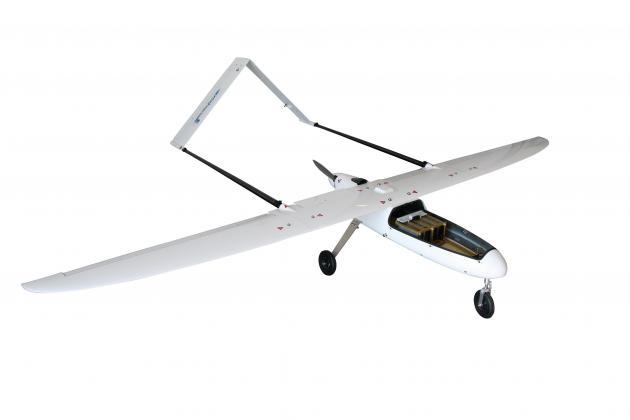
\includegraphics[width=0.7\textwidth]{penguin.jpg}
\caption{Aeronave modelo Penguin.} 
\label{fig:penguin}
\end{figure}

Para a realização da missão de varredura serão necessários algumas entradas a estação base, sendo elas, a quantidade de aeronaves a serem empregadas na missão, tempo de duração da missão, área a ser varrida e estratégia de varredura a ser utilizada, estratégias essas que serão apresentadas no Cap. \ref{Cap:Estrategia}.

Quando fornecidas todas as entradas corretamente, as rotas de voo serão definidas e carregadas nos VANTs e a missão terá inicio. O progresso da missão poderá ser acompanhada através da estação base e caso alguma embarcação seja identificada um alerta será lançado pela rede ate chegar a estação base visível ao operador da missão. Esse alerta será composto pela imagem da possível embarcação identificada pelo sistema, a localização geográfica do objeto e a hora na qual ele foi identificado.  






 

\mychapter{Características de uma Rede Multi VANTs}
\label{Cap:Requisitos}

As redes multi VANTs são uma evolução do sistema de comunicação formado por apenas um VANT e a base de controle, onde toda a troca de informações é realizada através de um \emph{link} entre as duas partes do sistema, situação em que há baixa confiabilidade no sistema de comunicação, pois caso esse \emph{link} seja interrompido por algum motivo, toda a comunicação seria impossibilitada. A rede multi VANTs é, então, proposta com intuito de aumentar o alcance e a confiabilidade do sistema através da adição de novos nós.

\cite{gupta2015survey} apresenta algumas das características de uma rede multi VANTs comparando-as à solução baseada em um único VANT, sendo elas:
\begin{itemize}
\item Escalabilidade
\item Capacidade de Sobrevivência
\item Velocidade da Missão
\item Complexidade do Controle
\item Economia de Energia
\end{itemize} 

\section{Escalabilidade}

Por definição uma rede multi VANTs é uma versão escalada da solução composta por um único VANT mais base de controle. Dessa forma, a adição de nós se torna uma operação comum a uma rede multi VANTs tornando-a uma solução escalável que pode variar o tamanho e, consequentemente, o alcance da rede dada as necessidades especificas da missão.

\section{Capacidade de Sobrevivência}

Como mencionado anteriormente, em uma solução formada por um único VANT mais base de controle, a rede é composta por apenas um \emph{link} e, caso esse seja interrompido, a comunicação entre esses dois nós será perdida. No entanto, dado que uma rede multi VANTs será formada por múltiplos nós e \emph{links}, em caso da perda de um nó a rede pode se reorganizar e garantir a sobrevivência da rede como um todo. 

Por exemplo, em uma rede composta por quatro nós em topologia \emph{mesh} como mostra a Figura \ref{fig:perdaNo}, no caso de falha do nó B, a comunicação entre os nós A e D poderá ser feita através do nó C, garantindo assim a sobrevivência da rede. 

\begin{figure} 
\center
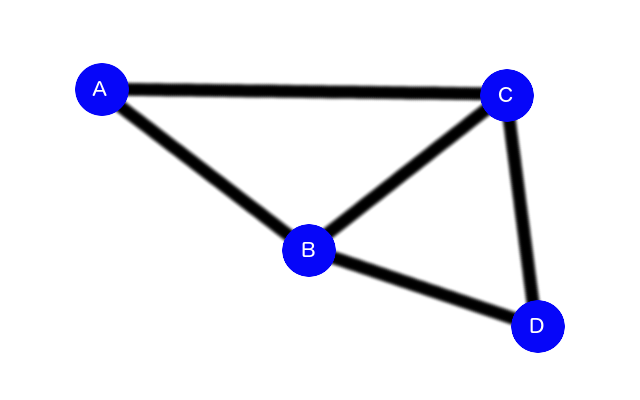
\includegraphics[width=0.7\textwidth]{perdaNo.png}
\caption{Exemplo de topologia de uma rede multi VANTs composta por 4 nós.} 
\label{fig:perdaNo}
\end{figure} 

\section{Velocidade da Missão}

A velocidade de realização de uma determinada missão será proporcional ao tamanho da rede multi VANT, quanto maior a quantidade de VANTs em uma determinada rede a ser utilizada para executar uma missão de varredura de área, menor será o tempo da missão. Por exemplo, pode-se dividir a área a ser varrida em sub-áreas que serão varridas simultaneamente, alocando cada um dos VANTs disponíveis para a missão a uma sub-área diferente. Por outro lado, a adição de um nó a uma rede resultará no aumento do custo da missão. Dessa forma, é importante analisar os benefícios do aumento de uma rede multi VANTs do ponto de vista financeiro. 

\section{Complexidade do Controle}

A complexidade do controle de uma rede composta por apenas um VANT e uma base de controle é baixa quando comparado ao cenário de uma rede multi VANTs. Quanto maior a quantidade de nós em uma rede maior será o custo computacional para controlar os nós e determinar os caminhos para realização da comunicação entre eles.

Outro ponto que aumenta ainda mais essa complexidade é a frequente mudança de topologia da rede, seja causada pela movimentação rápida dos nós, que se dá nas três dimensões, ou pela perda de nós devido a problemas de funcionamento ou fim da carga da bateria que alimenta o VANT.

\section{Economia de Energia}

Como VANTs possuem fonte de alimentação limitada, é importante garantir que a rede funcione da forma mais eficiente possível quanto ao consumo de energia, de tal forma que os nós possam permanecer ativos na rede pelo máximo de tempo possível. Caso a rede de comunicação consuma muita energia dos VANTs, será necessário a substituição de nós durante a execução de uma missão o que, consequentemente, aumentará o tempo necessário para a realização da mesma.\\

As características discutidas nesta sessão servirão de base para produção do protocolo de testes e, por fim, em trabalhos futuros para o desenvolvimento da arquitetura de rede a ser implementada no projeto SpaceVANT. 

\mychapter{Estratégia de Varredura}
\label{Cap:Estrategia}

Quando se utiliza apenas uma aeronave para realizar a varredura de uma área de impacto em busca de possíveis embarcações não autorizadas, pode-se utilizar de diferentes estratégias de voo, por exemplo, o método de varredura em espiral ou o método de varredura vai e volta \cite{ost2012search}. 

No primeiro método, a trajetória de voo é iniciada na extremidade da região e a aeronave percorrerá a área em espiral até o centro como mostra a figura \ref{fig:espiral}. 

\begin{figure} 
\center
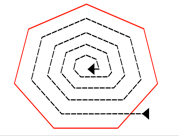
\includegraphics[width=0.5\textwidth]{espiral.png}
\caption{Método de Busca em Espiral.} 
\label{fig:espiral}
\end{figure} 

O segundo método realiza a varredura em linhas realizando curvas de 180 graus ao atingir a extremidade da área como mostra a figura \ref{fig:vaievolta}.

\begin{figure} 
\center
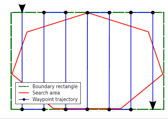
\includegraphics[width=0.5\textwidth]{vaievolta.png}
\caption{Método de Busca Vai e Volta.} 
\label{fig:vaievolta}
\end{figure} 

Em um cenário onde mais de um VANT será utilizado para a varredura de um área, há duas maneiras de acelerar a realização da missão, sendo elas realizar a inspeção com ou sem divisão em subárea. 

\section{Varredura sem Divisão em Subáreas}

Uma maneira de tomar proveito de uma rede multi VANTs para a varredura da área de impacto de foguetes seria realizar a missão varrendo a área por completo, mantendo os VANTs voando a uma mesma velocidade e espaçados igualmente realizando o mesmo percurso, como mostra a figura \ref{fig:semsubdivisao}. Ambos, velocidade e distância entre VANTs, serão relacionados ao ângulo de abertura da lente da câmera utilizada, a velocidade do processamento de imagem, altura e velocidade de voo.

\begin{figure} 
\center
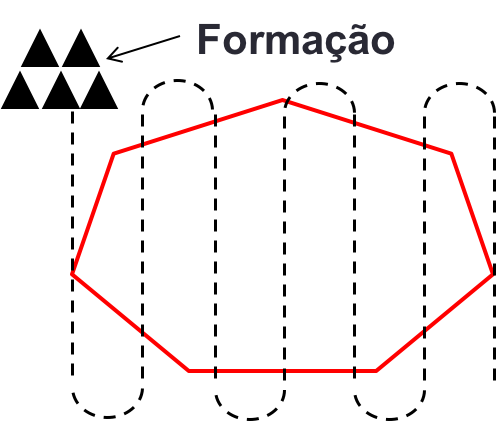
\includegraphics[width=0.5\textwidth]{semsubdivisao.png}
\caption{Varredura Vai e Volta sem Subdivisão de Área.} 
\label{fig:semsubdivisao}
\end{figure}

A utilização da estratégia sem divisão em subárea de varredura não há um considerável aumento de alcance da rede, pois os nós estarão sempre próximos. Por outro lado, em caso de perda de um nós o processo de reorganização é simples, bastando apenas aproximar os nós restantes. 

Uma decisão que pode ser tomada para aumentar o alcance da rede seria utilizar um nó de longo alcance e múltiplos nós de pequeno alcance, deixando a comunicação com a estação base a cargo do nó de maior alcance que funcionaria como \emph{hub} para os demais nós. Um ponto negativo dessa solução seria que caso o nó \emph{hub} perca conexão, os demais nós da rede também perderiam a conexão com a estação base. 

\section{Varredura com Divisão em Subáreas}

\begin{figure} 
\center
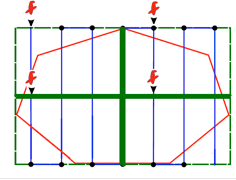
\includegraphics[width=0.5\textwidth]{comsubdivisao.png}
\caption{Varredura Vai e Volta com Subdivisão de Área.} 
\label{fig:comsubdivisao}
\end{figure}

Uma outra estratégia que poderia ser tomada seria dividir a área de varredura em subáreas de mesmo tamanho e utilizar os VANTs disponíveis para realizar a varredura de cada uma dessas subáreas como mostra a figura \ref{fig:comsubdivisao}. Nessa solução teríamos um aumento significante de alcance da rede, de modo que os pacotes serão transportados de nó em nó ate chegar a estação base ou nó de destino.

Em caso de perda de um dos nós da rede, a decisão a ser tomada para continuar a missão e garantir a varredura da área por completa não é tão trivial quando na estratégia de varredura sem divisão em subáreas, sendo necessário dividir novamente a área levando em consideração a área já varrida utilizando, por exemplo, a técnica proposta por \cite{marro2013path}.\\

Ambas as estratégias de varredura apresentadas nesta sessão possuem seus pontos negativos e positivos e a decisão de qual deles deve ser utilizada será função do operador do sistema de varredura. Na sessão a seguir serão discutidas as especificações técnicas do módulo Xbee adquirido pelo projeto.







\mychapter{XBee PRO S3B 900HP}
\label{Cap:Xbee}

O módulo XBee adquirido pelo projeto SpaceVANT para a implementação da rede multi VANTs foi o modelo XBee PRO S3B 900HP fabricado pela Digi Internation\textsuperscript{\texttrademark}. Esse capítulo descreve as especificações técnicas, método de configuração dos módulos e modos de operação como apresentado no guia de usuário do dispositivo. \cite{xbeemanuals3}

\section{Especificações Técnicas}

O guia do usuário do módulo XBee PRO S3B 900HP indica que o mesmo possui um alcance de comunicação de até 610 metros quando em ambiente interno ou urbano e transmitindo a 10 Kb/s. Quando o taxa de transmissão aumenta para 200 Kb/s, o alcance do módulo deve cair pela metade, ou seja, 305 metros. Para ambiente externo e com visada direta, o alcance será de 15.5 quilómetros transmitindo a uma taxa 10 Kb/s e 65 quilómetros quando transmitindo a uma taxa de 200 Kb/s.

O módulo, que ocupa uma volume de aproximadamente 3.66 cm\textsuperscript{3} e pesa entre 5 e 8 gramas, deve ser alimentado com uma fonte de 2.1 até 3.6 volts de corrente contínua, mas para fontes inferiores a 3.0 VDC a performance do módulo pode ser reduzida. A Banda de frequência de operação é selecionável via software e varia entre 902 e 927 MHz. Quanto a \emph{Interface} de dados, UART e SPI estão disponíveis para envio ou requisição de dados do módulo. O XBee PRO S3B 900HP também possui 15 pinos de I/O digital e 4 conversores analógico-digital de 10-bits distribuídos em 20 pinos físicos.

A respeito de rede e segurança, o módulo suporta redes de topologia \emph{mesh}, ponto-a-ponto, estrela ou \emph{peer-to-peer} utilizando Ids de 64 bits para endereçamento. Além disso, estão disponíveis 64 canais de comunicação que podem ser selecionados pelo usuário e opção de criptografia avançada padrão de 128 bits.

\section{Método de Configuração}

A respeito do processo de configuração dos módulos XBee, os parâmetros podem ser consultados e alterados de duas maneiras diferentes: forçando o aparelho a entrar em \emph{AT Command Mode}, solicitando ou enviando os valores do parâmetros do XBee atraves da \emph{interface} de dados, ou fazendo uso de do software XCTU disponibilizado pela Digi International\textsuperscript{\texttrademark}. 

\subsection{AT Command Mode}

A primeira maneira de configurar um módulo XBee seria fazer uso do modo \emph{AT Command Mode} enviando mensagens, de forma serial, requisitando valores de parâmetros ou solicitando alteração de algum parâmetro. É importante alertar que esse modo de configuração só é acessível através do uso da \emph{interface} UART.

Para forçar um modulo XBee a entrar em modo de configuração é necessário enviar um sequência especifica de caracteres, sendo essa sequencia composta por três caracteres de adição (+++). Após receber essa sequência, o módulo retornará `OK' indicando que o mesmo se encontra em \emph{AT Command Mode} aguardando algum comando, caso nenhum comando seja enviado em até um segundo, o modulo sai automaticamente do modo de configuração.

Um vez que o módulo já se encontra em \emph{AT Command Mode}, para solicitar o valor de um determinado parâmetro deve-se enviar a mensagem `AT' acompanhada da sigla do parâmetro que deseja-se obter o valor. Por exemplo, para verificar o valor do parâmetro \emph{Preamble ID} (HP), deve-se enviar o comando `ATHP' e aguardar o retorno do valor atual do parâmetro.

Para alterar o valor de um parâmetro em \emph{AT Command Mode}, deve-se enviar a mensagem `AT' acompanhada da sigla do parâmetro a ser modificado e o novo valor do parâmetro em hexadecimal, o uso de um espaço para separar a sigla do parametro do valor a ser atribuído é opcional. Caso deseja-se modificar o valor do \emph{Preamble ID} para 7FFF, envia-se `ATHP7FFF' ou `ATHP 7FFF'.

\subsection{XCTU Software}

Uma forma mais simples de visualizar e alterar os parâmetros de um módulo XBee é fazer uso do software fornecido pela fabricante do módulo, no caso do XBee PRO S3B 900HP, o XCTU (figura \ref{fig:xctu}) distribuido pela Digi International\textsuperscript{\texttrademark}.

Através do XCTU, pode-se procurar por módulos XBee conectados fisicamente ao computador onde a aplicação está rodando, visualizar e alterar os parâmetros do módulo conectado e até mesmo procurar os outros nós pertencentes a rede a qual o módulo está conectado, bem como visualizar e alterar os parâmetros dos outros nós da rede. 

Além de visualizar e editar paramêtros, o XCTU também possui um modo de console, onde pode-se enviar mensagens ao módulo conectado e visualizar o conteúdo dos mensagens que estão entrando e saindo do módulo, e um modo de visualização de rede, disponível apenas para módulos operando em \emph{API Mode}, onde são mostrados os nós que pertencem a rede do módulo conectado, bem como a topologia da rede.

O XCTU também possui algumas ferramentas para analise da qualidade da rede a qual o módulo XBee está conectada, por exemplo testes de força de sinal e \emph{throughput}, os quais foram utilizados para aferir a qualidade dos \emph{links} formados pelos XBee nesse trabalho.

\section{Modos de Operação}

O módulo XBee PRO S3B 900HP possui três possíveis modos de operação, sendo eles: \emph{Transparent Mode}, \emph{API Mode} e \emph{AT Command Mode}, utilizado exclusivamente para configuração do módulo e previamente explicado.

\subsection{Transparent Mode}

O \emph{Transparent Mode} é o modo de operação padrão do XBee e é obrigatório o uso da \emph{interface} UART ao utilizar desse modo. Quando funcionando em modo transparente, o módulo receberá dados, continuamente, através da porta UART e quando a quantidade de dados atingir o limite de \emph{bytes}, determinado na configuração do parâmetro \emph{Maximum RF Payload Bytes} (NP), os dados serão organizados em um \emph{frame} pelo próprio XBee e esse pacote é então enviado para o destinatário definido pelos parâmetros \emph{Destination Address High} (DH) e \emph{Destination Address Low} (DL). 

Apesar da facilidade de uso, esse modo de operação é indicado apenas para uso em redes com topologia ponto-a-ponto, onde o destinatário dos pacotes não varia com frequência, pois para mudar o destinatário de um pacote nesse modo de operação será necessário entrar em modo de configuração e alterar múltiplos parâmetros para cada envio. Sendo assim, esse modo nao é adequado para a implementação de uma rede multi VANTs onde um mesmo pacote podera ser enviado para múltiplos nós na rede, por exemplo.

\subsection{API Mode}

Diferentemente do \emph{Transparente Mode}, onde o XBee realiza a operação de criação do \emph{frame} que será transmitido, no \emph{API Mode} o módulo já recebe o frame contendo todas informações como destinatário e tipo de dado, por exemplo, e apenas transmite o \emph{frame} recebido de acordo com as informações do mesmo. Esse modo é compatível com ambas as \emph{interfaces} UART e SPI.

A estrutura do \emph{frame} a ser recebido pelo XBee está ilustrada na figura \ref{fig:apiframe} e contem quatro campos principais. O primeiro \emph{byte} do frame indica apenas o início do mesmo, seguido por dois \emph{bytes} que irão indicar o tamanho do frame, sem contar o \emph{byte} que é utilizado para garantir a integridade do \emph{frame} através de um operação \emph{chesksum} e, por fim, a maior porção do \emph{frame} contém o dado que está sendo transmitido e o identificador daquele tipo de dado.

Esse modo de operação é indicado para redes com topologia \emph{mesh}, pois o destinatário no \emph{frame} está indicado dentro do mesmo, sem a necessidade de configurar o módulo a cada novo envio. Sendo assim, o \emph{API Mode} se apresenta como um modo de operação compatível com o contexto de um rede multi VANTs.\\

Apresentadas as especificações técnicas do módulo XBee PRO S3B 900HP, os modos de operação disponíveis e o ambiente de configuração e testes XCTU, o próximo capítulo descreve o procedimento dos testes realizados para avaliar a viabilidade desse módulo na implementação de uma rede multi VANTs, bem como os componentes utilizados nos testes. 

\begin{figure} 
\center
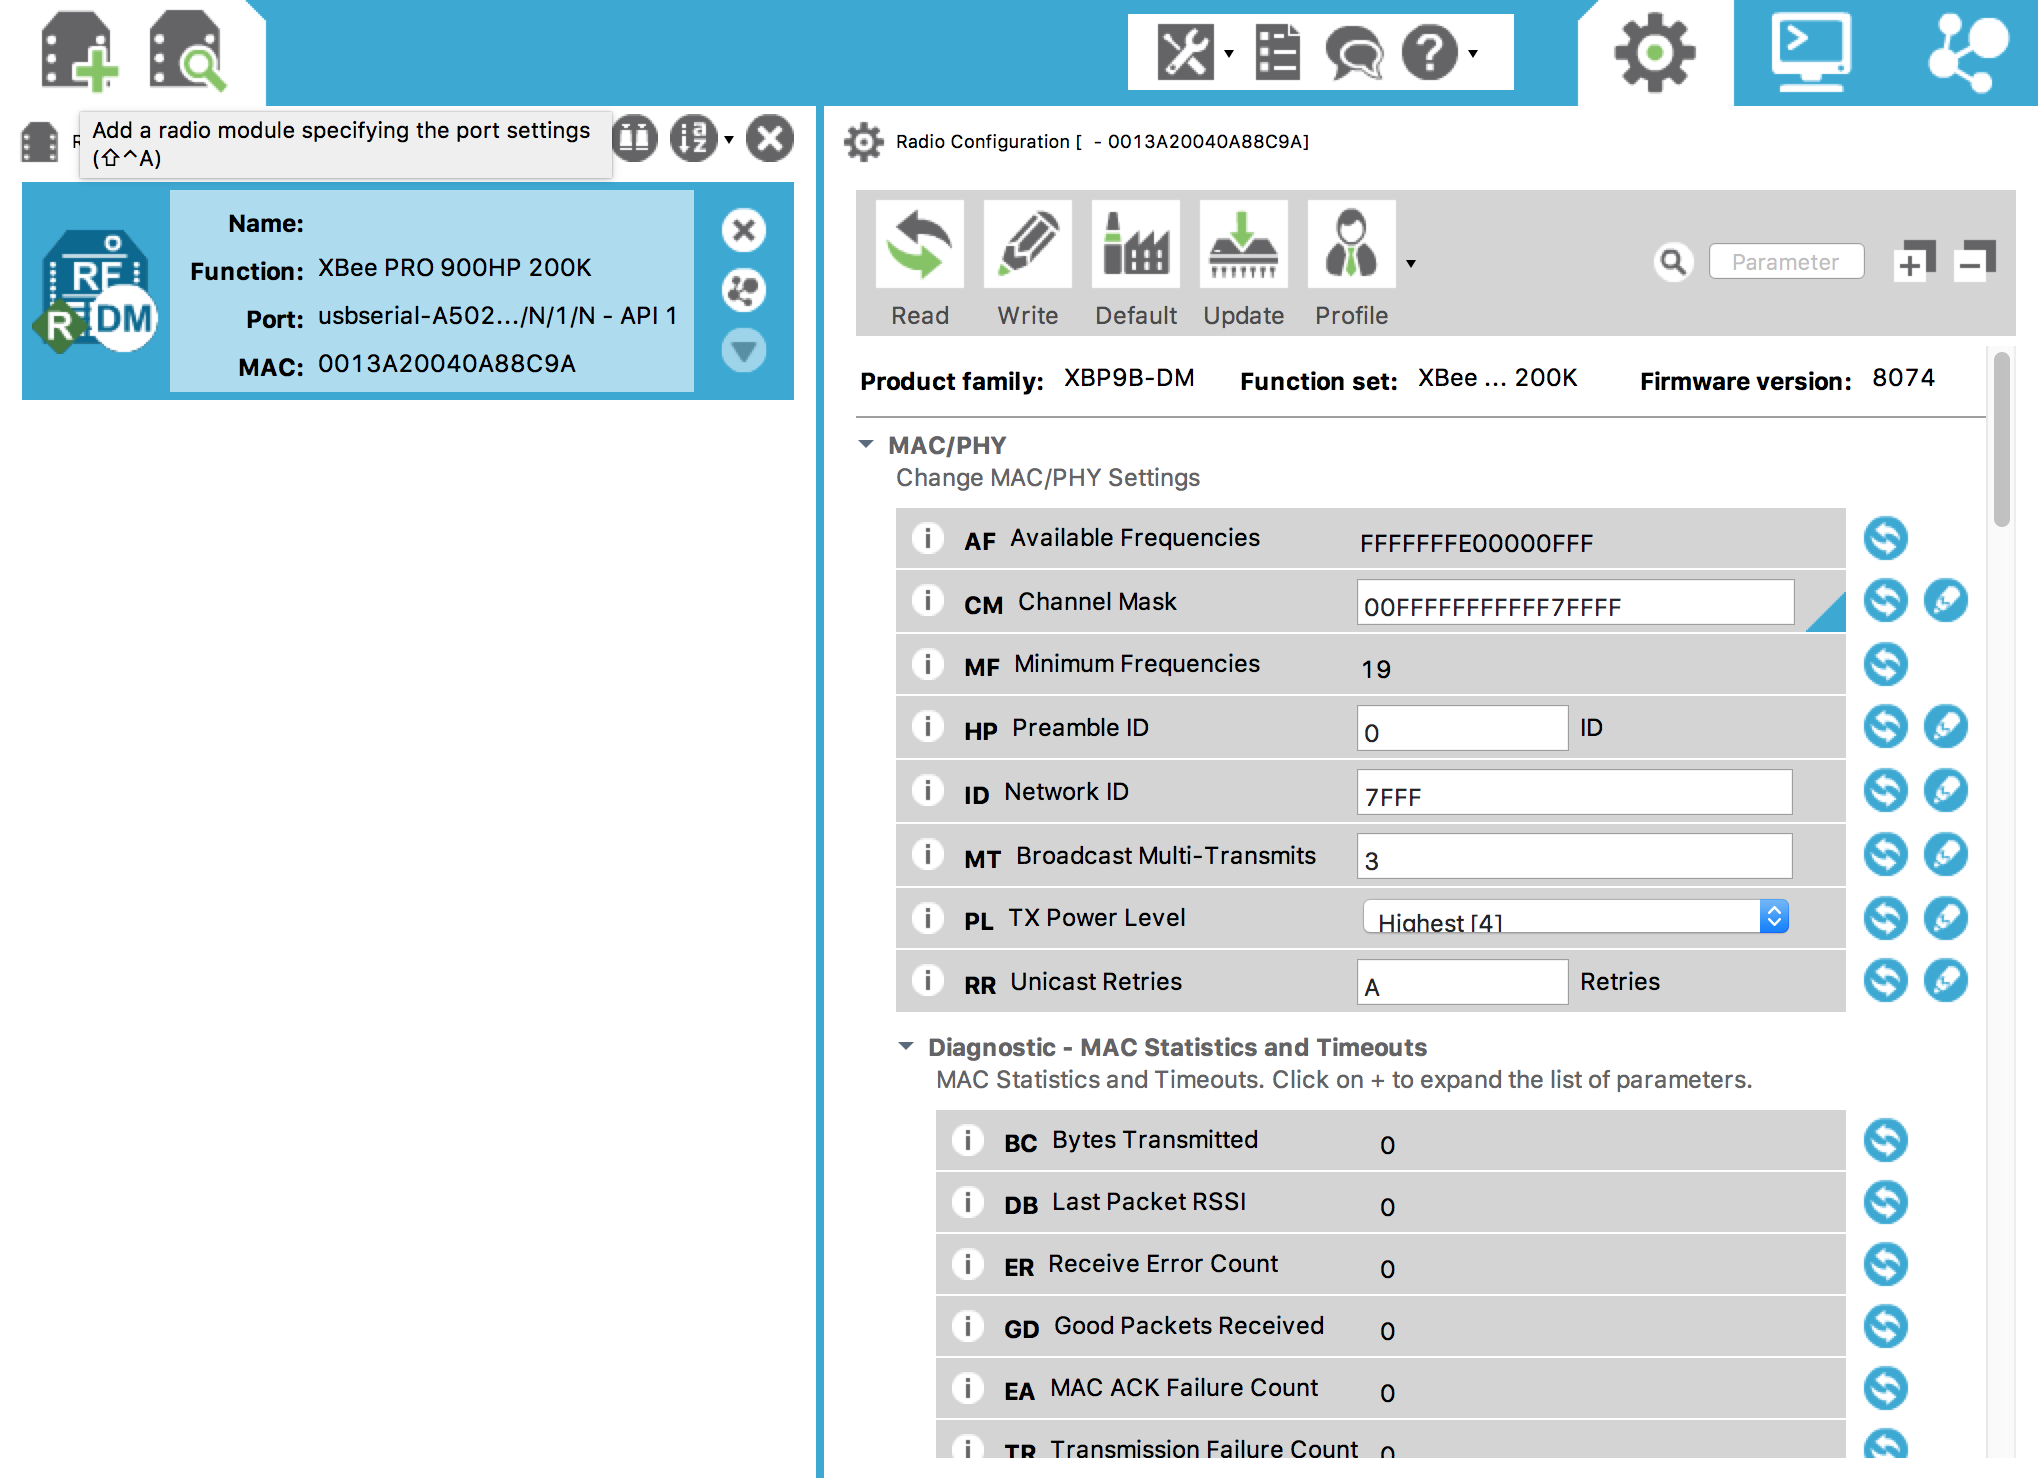
\includegraphics[width=0.7\textwidth]{xctu.png}
\caption{Pagina inicial do software XCTU.} 
\label{fig:xctu}
\end{figure}

\begin{figure} 
\center
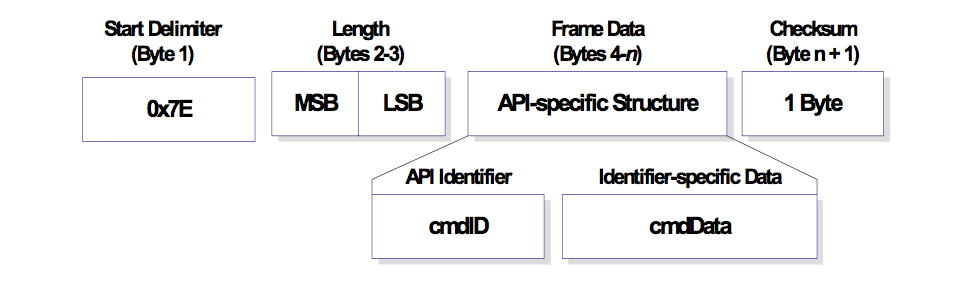
\includegraphics[width=0.7\textwidth]{apiframe.png}
\caption{Estrutura do \emph{frame} no modo API.} 
\label{fig:apiframe}
\end{figure}

\mychapter{Procedimento Experimental}
\label{Cap:Procedimento}

Esse capítulo descreve os dispositivos e a metodologia utilizada na execução dos experimentos, o cenário onde esses experimentos formam realizados e, por fim, os experimentos realizados para aferir parâmetros de funcionamento dos módulos XBee PRO S3B 900HP.

\section{Tecnologias Utilizadas}

Além do módulo XBee PRO S3B 900HP (fig \ref{fig:xbeepro}), foram utilizados na execução dos experimentos: módulos XBee \emph{Explorer}, aeronaves \emph{Phantom 3 Standard}, o \emph{software} XCTU utilizado para a realização dos testes e uma fonte de alimentação externa para alimentar o conjunto módulo XBee + XBee \emph{Explorer}.

As especificações técnicas, bem como o modo de funcionamento, dos módulos XBee já foram discutidos no capítulo \ref{Cap:Xbee}. Os demais materiais utilizados serão descritos a seguir.

\begin{figure}[h!] 
\center
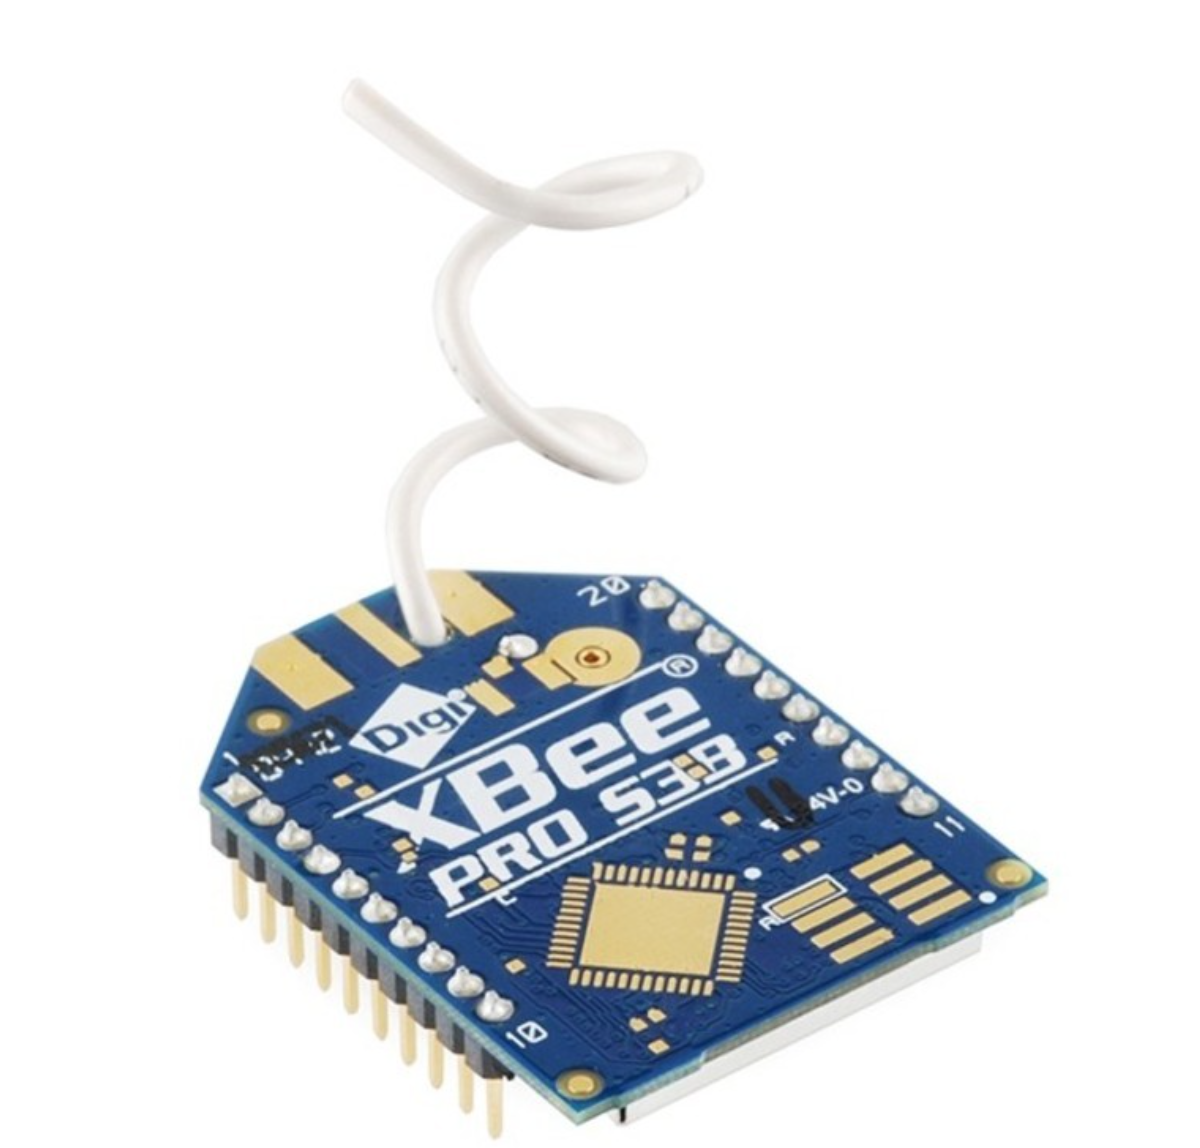
\includegraphics[width=0.7\textwidth]{xbeepro.png}
\caption{Módulo XBee PRO S3B 900HP.} 
\label{fig:xbeepro}
\end{figure}

\subsection{XBee \emph{Explorer}}

O XBee \emph{Explorer} é a \emph{interface} de \emph{hardware} utilizada para conectar um módulo XBee a outros dispositivos, como por exemplo um computador. O módulo adquirido pelo projeto, como mostra a figura \ref{fig:xbeeexplorer}, possui duas formas de acesso ao módulo XBee acoplado a ele, sendo essas uma porta micro usb, utilizada para alimentação e comunicação, ou um conjunto de pinos contendo Rx, Tx, \emph{reset} e os pinos a serem utilizados para alimentação.

Apesar de da voltagem de alimentação dos módulos XBee ser de +3.3 volts, o XBee \emph{Explorer} deve ser alimentado com uma fonte que forneça +5 volts, que é reduzida para a voltagem de alimentação requerida pelo módulo XBee através da circuitaria do \emph{Explorer}.

\begin{figure}[h!] 
\center
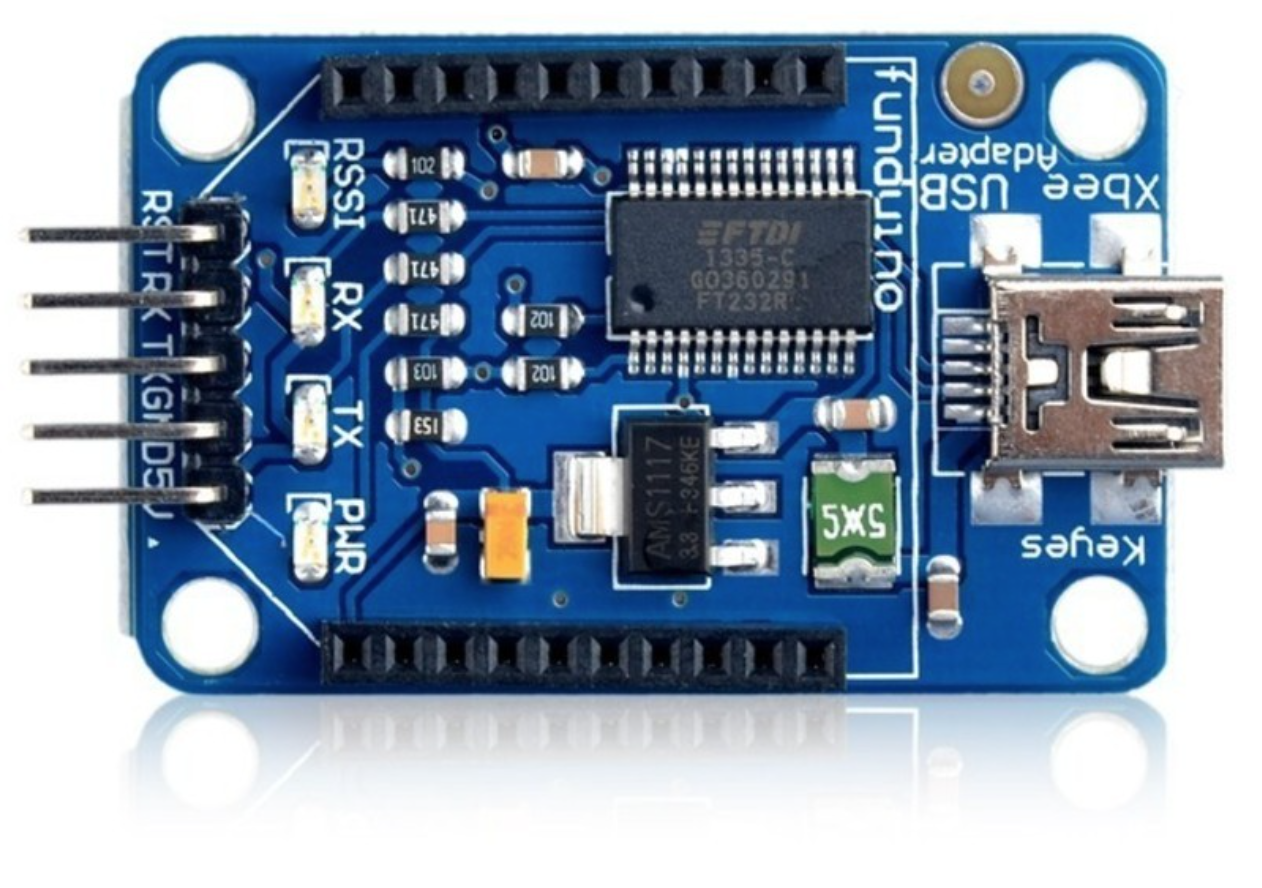
\includegraphics[width=0.7\textwidth]{xbeeexplorer.png}
\caption{XBee \emph{Explorer}.} 
\label{fig:xbeeexplorer}
\end{figure} 

\subsection{Phantom 3 Standard}

Outro dispositivo de grande importância para a realização dos experimentos foram os quadrirrotores do modelo \emph{Phantom 3 Standard} (figura \ref{fig:phantom}) adquiridos pelo projeto e utilizados para variação e medição da distância entre os nós da rede \emph{mesh} formada para a realização dos teste de performance.

As aeronaves são controladas utilizando controle remoto que as acompanha e um \emph{smartphone} rodando o aplicativo DJI Go, que da suporte visual para a operação das aeronaves. Parâmetros como altitude de voo, velocidade vertical e horizontal, nível de bateria, distância entre a aeronave e o operador, entre outros, estão sempre de fácil acesso visual bem como a imagem capturada pela câmera embarcada que é transmitida em tempo real para o operador. 

\begin{figure}[h!] 
\center
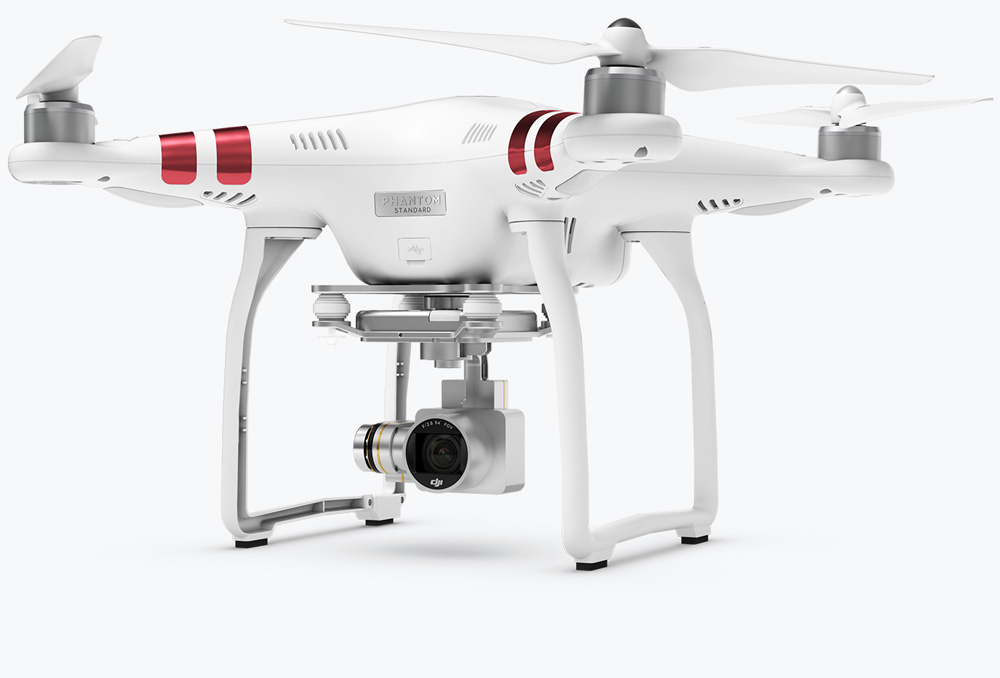
\includegraphics[width=0.7\textwidth]{phatom.jpg}
\caption{Aeronave Phantom 3 \emph{Standard}.} 
\label{fig:phantom}
\end{figure}

\subsection{XCTU}

O XCTU, bevemente apresentado no capítulo \ref{Cap:Xbee}, é o \emph{software}, disponibilizado pela fabricante dos módulos XBee, utilizado para configuração dos dispositivos e que também possui algumas ferramentas para analise da qualidade da rede formada. Ferramentas essas que foram utilizadas nesse trabalho para aferir a qualidade da rede, em especial o teste de força de sinal e o de taxa de transmissão (\emph{throughput}).

As figuras \ref{fig:rangeTest} e \ref{fig:throughput} apresentam, respectivamente, as telas dos testes de força de sinal e taxa de transmissão disponíveis no \emph{software} XCTU.

\begin{figure}[h!] 
\center
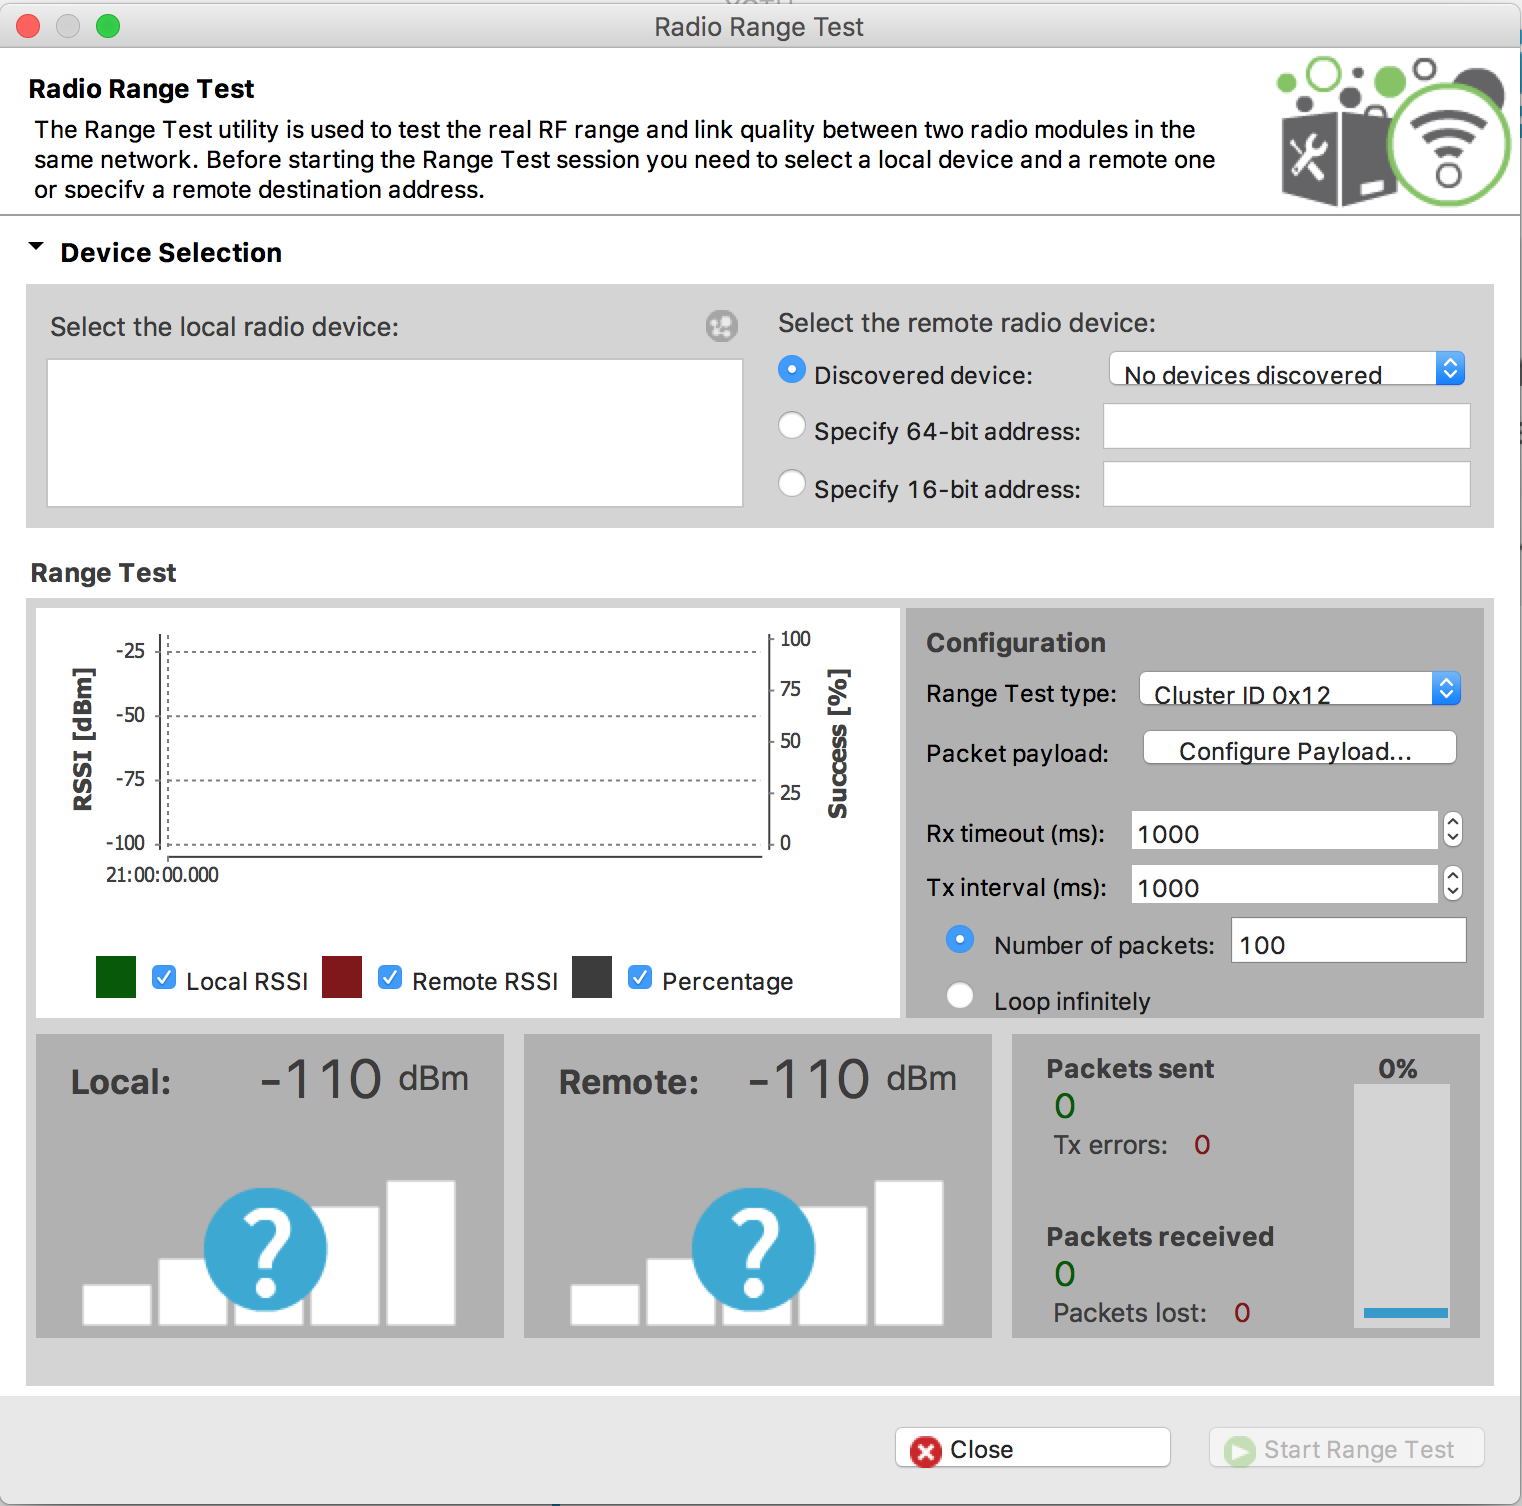
\includegraphics[width=0.7\textwidth]{RangeTest.png}
\caption{Tela do teste de força de sinal.} 
\label{fig:rangeTest}
\end{figure}

\begin{figure}[h!] 
\center
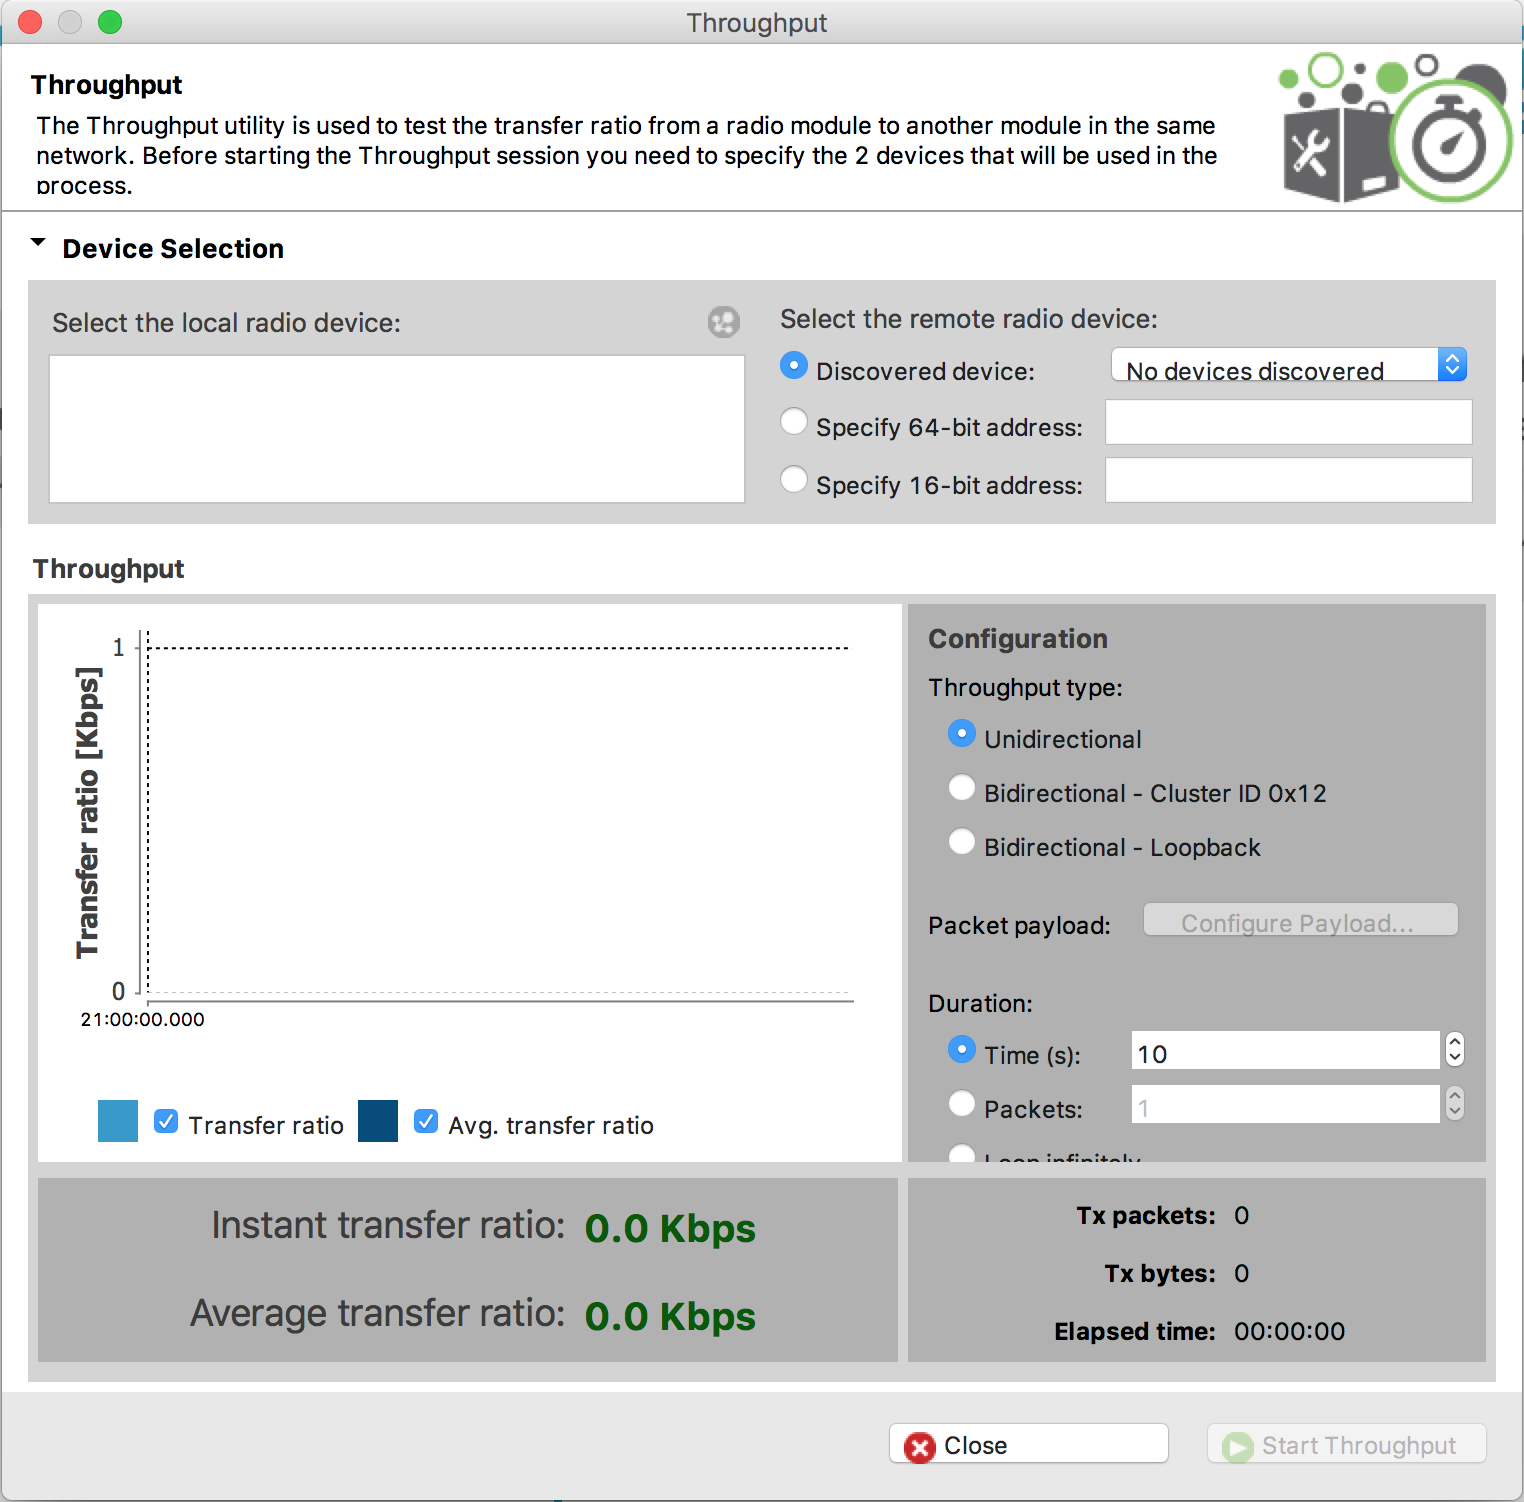
\includegraphics[width=0.7\textwidth]{ThroughputTest.png}
\caption{Tela do teste de taxa de transmissão (\emph{throughput}).} 
\label{fig:throughput}
\end{figure}

\section{Local dos Experimentos}

O local ideal para a realização dos experimentos seria o local onde o sistema final seria utilizado, ou seja, o próprio Centro de Lançamento Barreira do Inferno (CLBI), pois os testes refletiriam as condições especificas de interferência e meio de comunicação onde a rede multi VANTs será operada.

Infelizmente, devido a indisponibilidade de tempo e acesso, os testes de campo aqui apresentados foram realizados em sua maioria no campo central da Universidade Federal do Rio Grande do Norte (UFRN), o que pode ser considerado um ambiente urbano e pode apresentar níveis de interferência de sinal maiores que o ambiente onde a rede será de fato operacionalizada. 

\section{Experimentos Realizados}

No intuito de aferir a qualidade dos \emph{links} e, consequentemente, a rede a qual eles fazem parte, no contexto de um rede multi VANTs, foram realizados múltiplos testes de força de sinal e taxa de transmissão para diferente cenários, sendo eles:

\begin{itemize}
\item Teste de chão
\item Teste em ar a distância fixa
\end{itemize} 

\subsection{Teste de Chão}

Para a realização dos testes de chão, o conjunto de equipamentos necessários (módulo XBee + XBee \emph{Explorer} + bateria portátil) foram afixados ao \emph{Phantom 3 Standard} com o auxílio de fita colante do tipo \emph{silver tape}, como mostra a figura \ref{fig:conjExp}, e um outro módulo XBee foi conectado ao um \emph{notebook} dotado do \emph{software} XCTU, através do XBee \emph{Explorer}.

O aeromodelo, embarcado com os equipamentos requeridos, foi então posicionado em diferentes pontos do campo e os testes de força de sinal e taxa de transferência, disponíveis no XCTU, foram executados e seus resultados armazenados para analise. Os testes foram realizados 5 vezes para cada distância e a média desses cinco resultados foi considerado para análise de desempenho. 
 
\subsection{Teste em Ar a Distância Fixa}

Assim como nos testes de chão, com o auxilio de fita colante, um módulo XBee, um XBee \emph{Explorer} e uma bateria portátil foram afixados ao aeromodelo (fig. \ref{fig:conjExp}) e um outro módulo XBee foi conectado, através do XBee \emph{Explorer}, a um \emph{notebook} dotado do \emph{software} XCTU. 

Uma vez que todos os equipamentos estavam devidamente conectados, a aeronave \emph{Phantom} foi guiada, através do controle com o auxilio do supervisório DJI Go, para uma determinada região em ar para a realização dos testes. Para cada conjunto de testes, foi definida uma altitude e apenas a distância horizontal entre os módulos XBee foi variada.

Mais uma vez, os testes de força de sinal e taxa de transferência, disponíveis no XCTU, foram executados cinco vezes para cada distância e seus resultados armazenados para análise. 

\begin{figure} 
\center
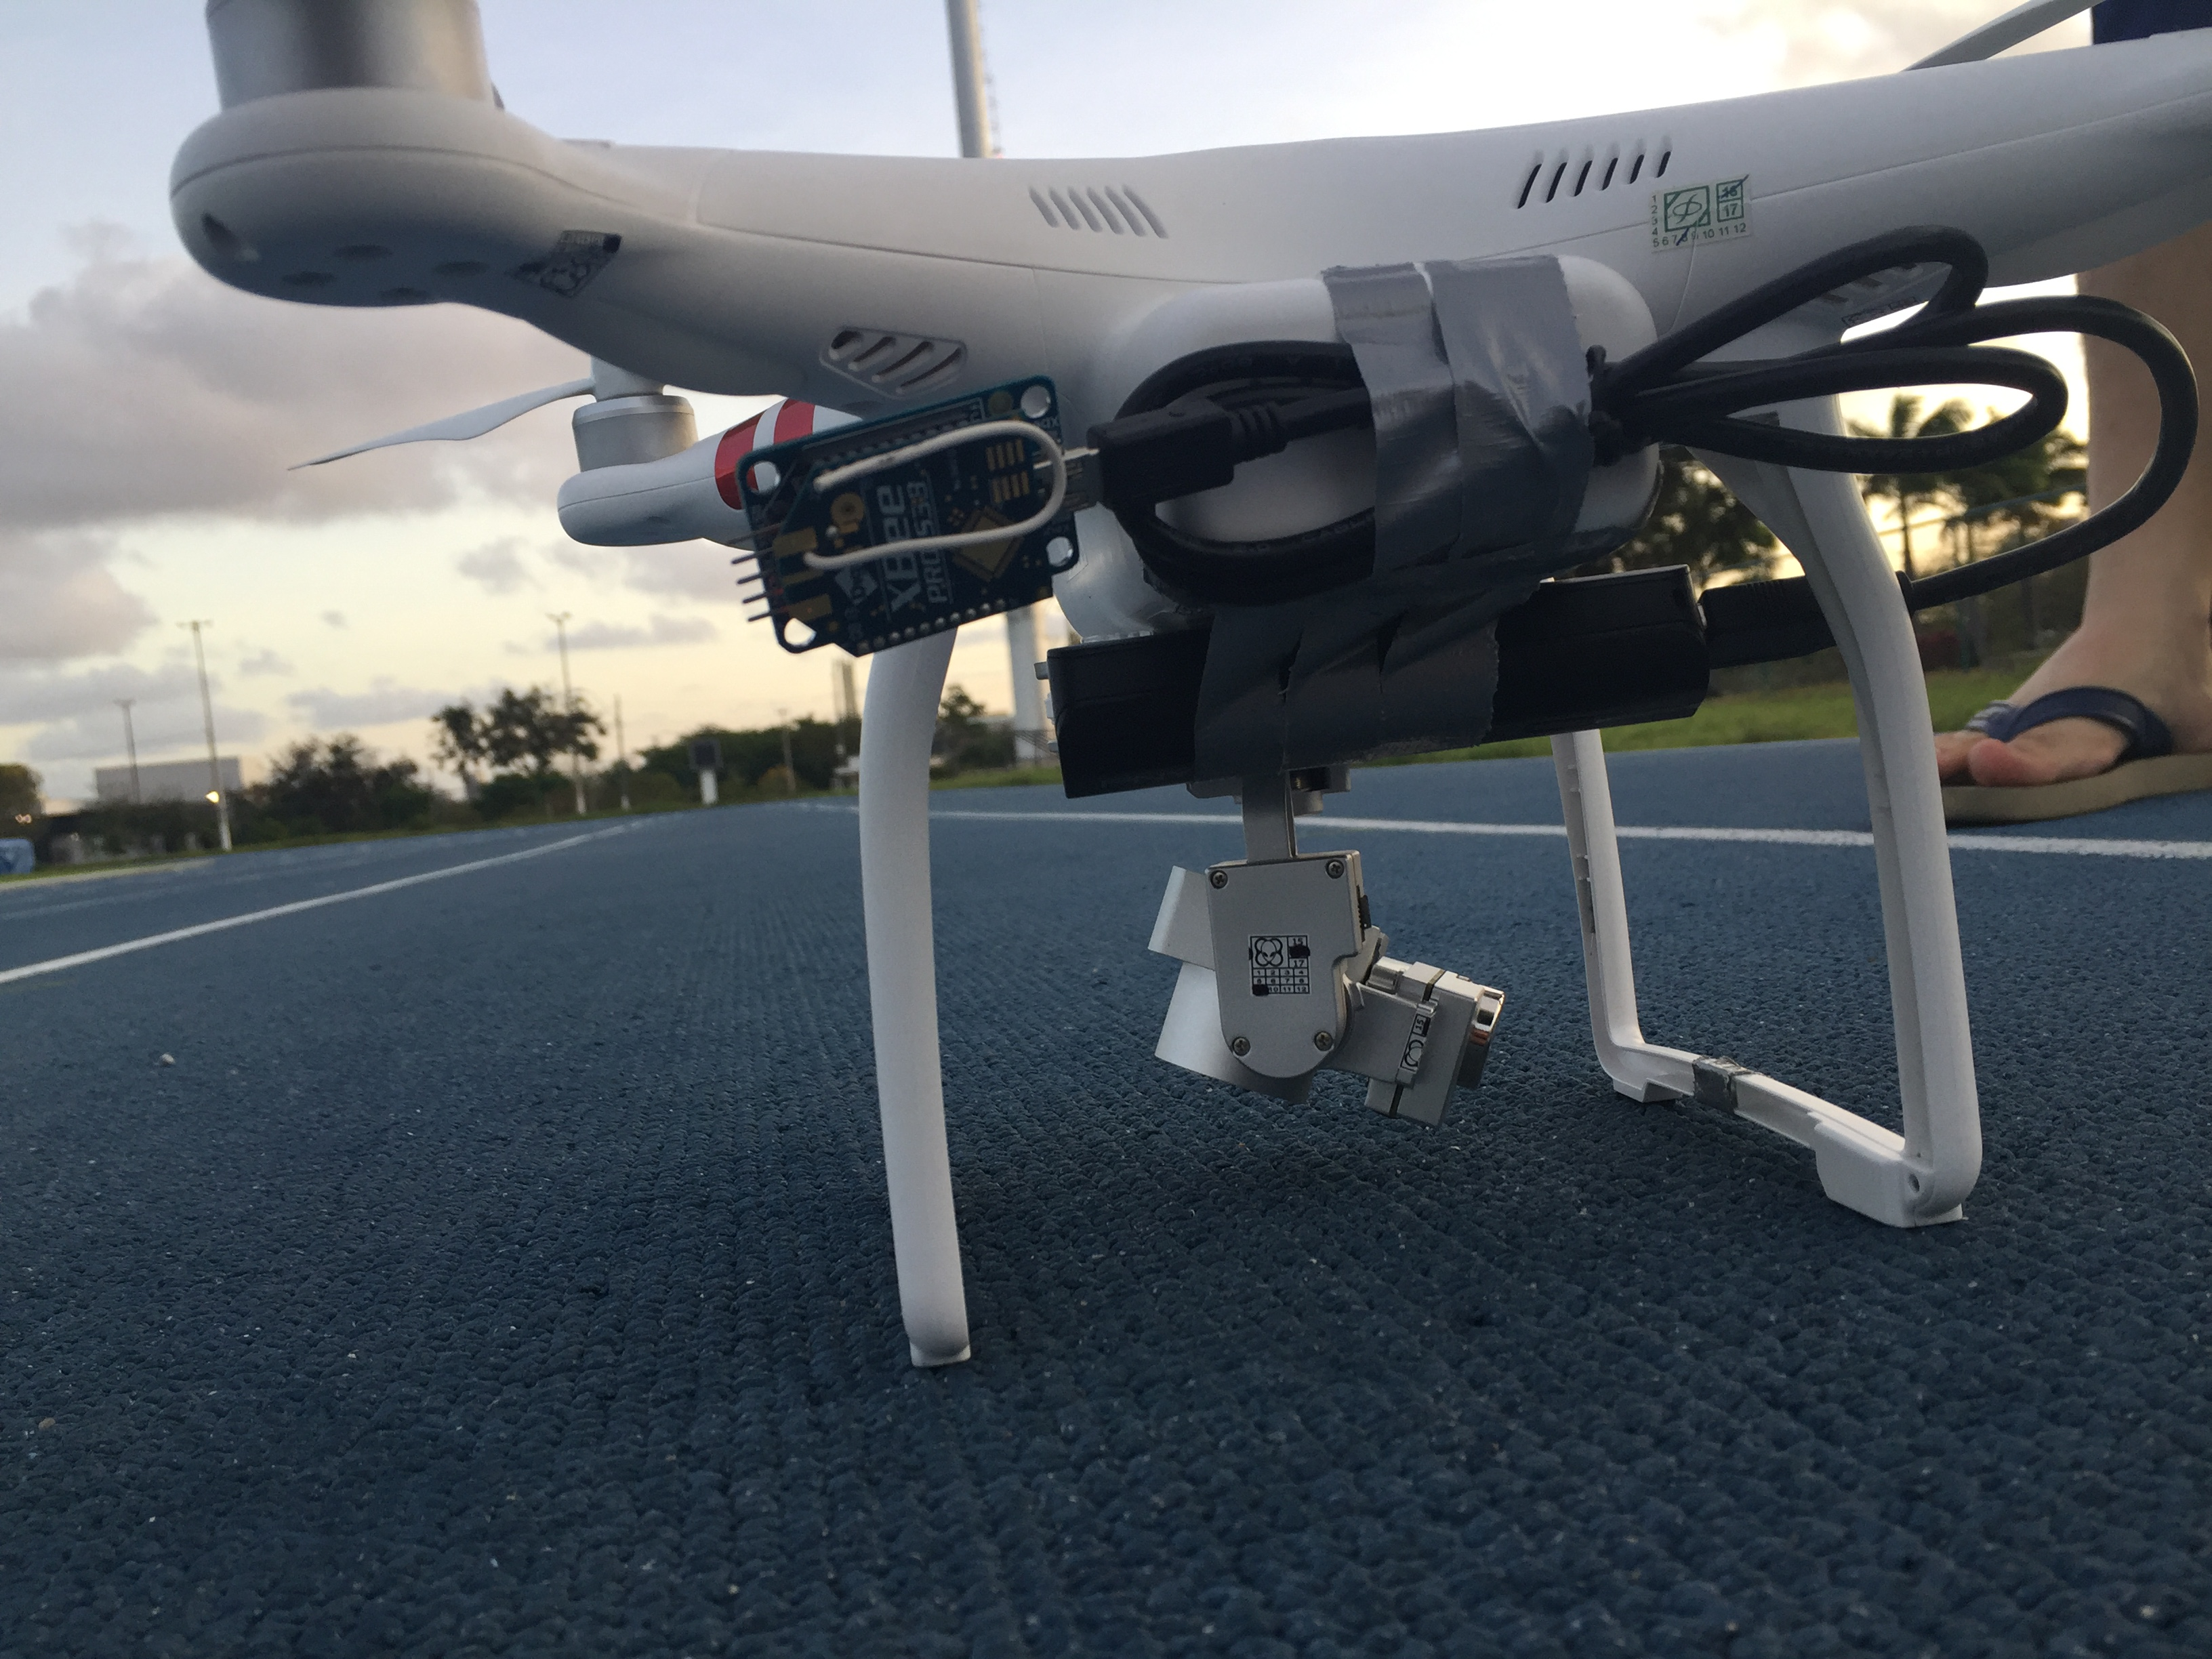
\includegraphics[width=0.7\textwidth]{conjExp.jpg}
\caption{\emph{Phantom 3 Standard} preparado para experimentos.} 
\label{fig:conjExp}
\end{figure}

\mychapter{Resultados Experimentais}
\label{Cap:Resultados}

Antes mesmo de testar a qualidade da comunicação dos módulos XBee em chão, foram realizados testes de comportamento do aeromodelo \emph{Phantom} quanto a possível interferência que a rede formada pelos XBees poderia causar na comunicação entre o mesmo e o controle remoto, afim de garantir a integridade de ambos os equipamentos envolvidos. Certificou-se, então, que o funcionamento da aeronave em nada era afetado com a presença da rede XBee.

\section{Teste em Solo}

Para a análise da qualidade da rede XBee em solo, foram realizados três testes de potência do sinal a três diferente distâncias, sendo elas 50, 100 e 236. Para cada teste foram enviados 40 pacotes de dados com metade da capacidade máxima de \emph{payload}, ou seja, 32 \emph{bytes}. Como mostra a Figura \ref{fig:SuccessChao}, a taxa de sucesso de envio de pacotes cai de aproximadamente 95 por cento para 5 por cento entre as distâncias de 100 e 236 metros, praticamente eliminando o \emph{link} de comunicação entre os dois nós da rede.

Para os testes realizados com 236 metros de afastamento entre os nós, nas quarenta tentativas de envio de pacote entre os nós da rede, trinta e oito delas acusaram \emph{TX Errors}, o que significa que o nó remetente não foi capaz de criar o \emph{link} de comunicação com o nó destinatário do pacote, resultando assim em apenas duas transmissões de dados bem sucedidas, resultando na taxa de sucesso de 5 por cento.

Quanto ao teste da taxa de transmissão de dados, foram realizados apenas dois testes sendo o primeiro com 50 metros de afastamento entre os nós e o segundo com 100 metros. Para a terceira distância, sendo essa 236 metros, foi impossível a realização do teste de taxa de transferência devido a má qualidade de comunicação. Os resultados desses dois testes podem ser vistos na Figura \ref{fig:ThroughputChao}.

O resultado de ambos os testes de força de sinal e taxa de transmissão não corresponderam ao esperado. Como os testes foram realizados no campo central da UFRN, considera-se área urbana, esperava-se que os módulos tivessem um desempenho próxima à indicada no manual do equipamento, que seria um alcance de aproximadamente 610 metros com uma taxa de transmissão de 10 kbps, ou 305 metros com uma taxa de transmissão de 200 kbps. Em contra partida, a comunicação entre os nós já foi comprometida à aproximadamente 235 metros e a taxa de transmissão alcançada nos testes a menor distância não ultrapassou os 6 kbps. 

\begin{figure} 
\center
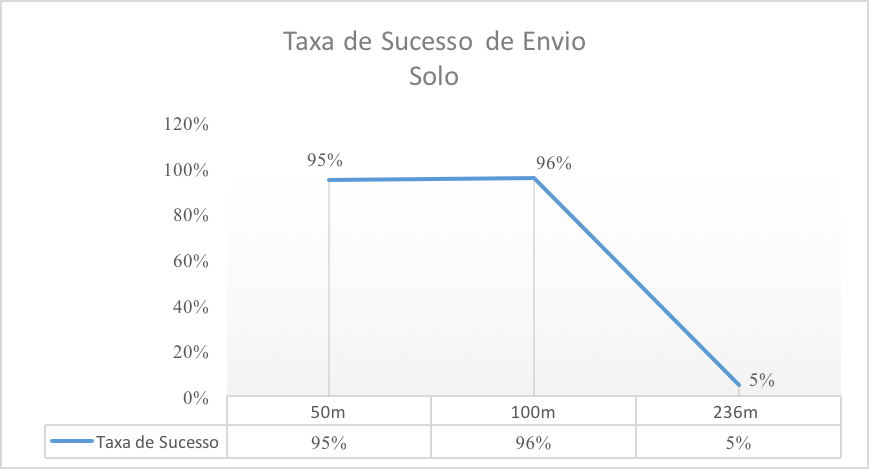
\includegraphics[width=0.7\textwidth]{sucessRateChao.png}
\caption{Gráfico da taxa de sucesso de envio \emph{versus} distância entre os dois nós da rede XBee.} 
\label{fig:SuccessChao}
\end{figure} 

\begin{figure} 
\center
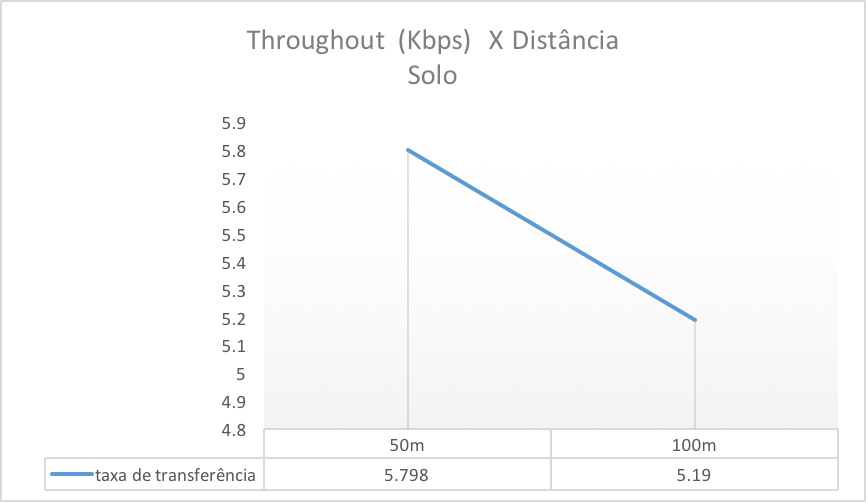
\includegraphics[width=0.7\textwidth]{throughputResultChao.png}
\caption{Gráfico da taxa de transmissão de envio \emph{versus} distância entre os dois nós da rede XBee.} 
\label{fig:ThroughputChao}
\end{figure}
 
\section{Teste em Ar a Distância Fixa}

Os resultados obtidos nos testes realizados em ar foram consistentes com as especificações do módulo XBee. Foram realizados testes de força de sinal e taxa de transmissão com afastamentos entre os nós de 50 até 700 metros e altitude fixada em 80 metros, sendo de 50 a 400 metros com aumentos de 50 metros e de 400 a 700 metros com aumentos de 100 metros.

Para todos os testes realizados, todos os quarenta pacotes enviados, por teste, foram transmitidos com sucesso entre o nó remetente e o nó destinatário, resultando em um taxa de sucesso de envio de cem por cento em toda essa faixa de distância, que vai de 50 até 700 metros de afastamento entre os nós.

Apesar da excelente taxa de sucesso, a potência do sinal transmitido entre os nós teve um comportamento inesperado. Em um cenário de afastamento entre os nós, o valor de RSSI (em português, indicador de potência de sinal recebido) deveria decaí proporcionalmente ao afastamento os nós, resultando em um \emph{link} de conexão mais fraco entre os nós. No entanto, nos resultados do experimento esse indicador varia com a distância de afastamento de forma irregular. Esse comportamento pode ser verificado na figura \ref{fig:RangeChao}, onde é possível observar que o valor apresentado decai até os 350 metros de afastamento, onde tem uma repentina subida, decai mais um pouco até os 400 metros e começa a aumentar novamente. 

Quanto a taxa de transmissão, nos testes realizados em ar, os módulos XBee se comportaram de forma altamente inesperada, variando a taxa de transmissão de dados bruscamente, inicialmente, por razão indefinida. A Figura \ref{fig:ThroughputAr} apresenta os resultados obtidos, onde pode-se observar que a taxa de transmissão tem um aumento repentino a partir dos 350 metros de afastamento entre os nós e permanece aumentando com o afastamento, chegando a atingir um \emph{throughput} de aproximadamente 30 kbps.

Apesar do comportamento inesperado, os testes em ar foram condicentes com as especificações do módulo. Já a respeito do comportamento inesperado, testes preliminares apontaram que fatores como o tamanho do pacote a ser enviado, bem como \emph{baudrate}, possuem grande efeito tanto na taxa de sucesso da comunicação quanto na taxa de transmissão desses pacotes, o que leva a acreditar que a taxa de transmissão de 200 kbps apresentada no manual do módulo XBee poderá vir a ser alcançada mudando alguns parâmetros de configuração do módulo e características do pacote a ser enviado.\\

Os resultados obtidos nesse trabalho foram importantes para direcionar os testes futuros a serem realizados dentro do projeto SpaceVANT e produzir um protocolo de testes mais formalizado levando em consideração os parâmetros que afetam a qualidade da conexão na rede XBee.   

\begin{figure} 
\center
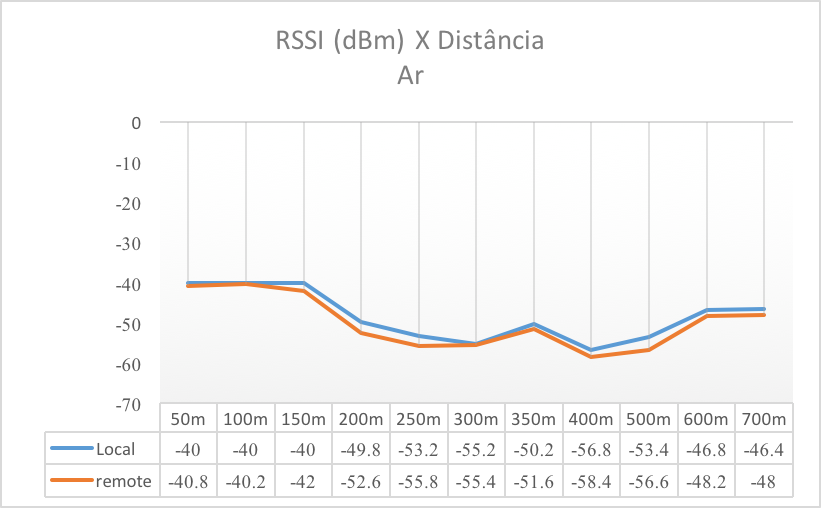
\includegraphics[width=0.7\textwidth]{rangeResultAr.png}
\caption{Gráfico do RSSI local e remoto \emph{versus} distância entre os dois nós da rede XBee.} 
\label{fig:RangeChao}
\end{figure}

\begin{figure} 
\center
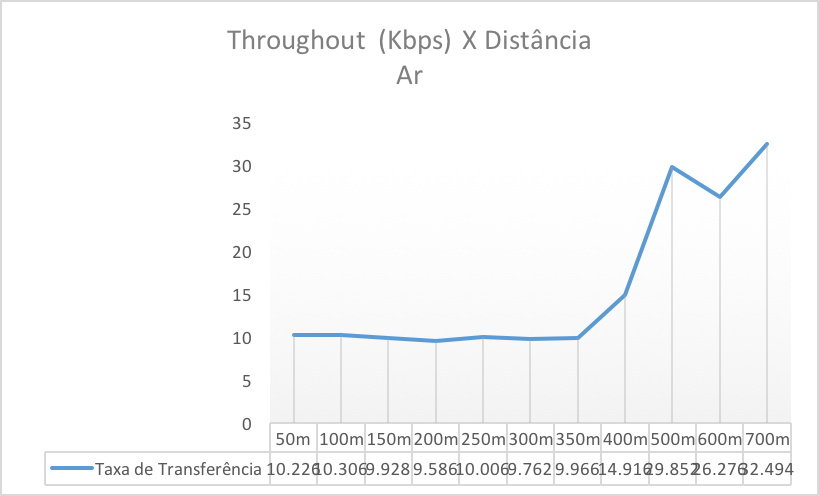
\includegraphics[width=0.7\textwidth]{throughputResultAr.png}
\caption{Gráfico da taxa de transmissão de envio \emph{versus} distância entre os dois nós da rede XBee.} 
\label{fig:ThroughputAr}
\end{figure}












\mychapter{Conclus\~{a}o}
\label{Cap:conclusao}



% Refer\^{e}ncias bibliogr\'{a}ficas (geradas automaticamente)

\addcontentsline{toc}{chapter}{Refer\^{e}ncias bibliogr\'{a}ficas}
\nocite{*}
\bibliography{bibliografia}


\appendix

% Ap\^{e}ndice A
%\include{apendice/apendice}

% Ap\^{e}ndice B
%\include{apendice/apendiceB}

% Ap\^{e}ndice C
%\include{apendice/apendiceC}

\end{document} 